\documentclass[../physical_computing.tex]{subfiles}

\begin{document}

\chapter{Starting point}

\section{What is Physical Computing?}
\label{sec:what_is_physical_computing}

Science and Engineering all about making connections between nature and mathematics. A successful scientific theory makes a connection between the behaviour of some real world hardware in an experiment and the properties of an abstract mathematical system that reproduces what is seen in that experiment. The starting point is observations about the real world hardware, and the end point is a mathematical model exhibiting the same behaviour, and perhaps predictive power. In engineering it is the same process in reverse. You start with an abstract idea that you want a real world system to replicate, and your end point is the realisation of that real world system - a machine. So science and engineering are both about relationships between nature and mathematics. In order to do either effectively, it is sometimes best to start from the simplest building blocks. Conceptually, the simplest abstract system is one that can only be in two states, say true or false. A two state system like this is called a bit. Bits turn out to be the basic currrency of computers that are some of the most sophisticated machines that engineers have produced, and have started the information revolution. In this book, we will be mostly concerned at first with bits and how to represent them using electronic circuits. We will catch glimpses of what those electronic circuits can do for science, and how they can be used as tools for building better abstract models of reality, also known as scientific theories.

The manipulation of these representations of bits using circuits is called digital signal processing (DSP). In classical digital signal processing, ranges of voltages on wires are used to represent the values of bits. For example, in 3.3V CMOS logic, the convention is that any voltage between $\rm 2.0\,V$ and $\rm 3.3\,V$ represents logic $1$, or true, any voltage between $\rm 0.0\,V$ and $\rm 0.8\,V$ represents logic $0$, or false. Just as the bits themselves are represented by classical voltage ranges, the operations on the bits are represented by circuits. For example, the simplest abstract digital operation I can think if is NOT, where if the input is a $0$ then the output is a $1$ and vice versa. An implementation of a NOT in a digital circuit must generate an output between $\rm 0.0\,V$ and $\rm 0.8\,V$ from an input between $\rm 2.0\,V$ and $\rm 3.3\,V$, and vice versa. Though of course digital circuits have become incredibly sophisticated, we shall show that all of them are made up of three basic circuit elements - gates, registers and oscillators. So the fundamental building blocks of classical computers are fewer in number than the fundamental building blocks of the Universe in particle physics!

In the first part of this book, we will learn to design and build digital circuits out of these three basic building blocks. The tasks that can be carried out by these circuits will be very simple, but I hope that by understanding the basic principles of how these blocks are combined, you will be able to see how these ideas can be generalised to far more complex systems. Forty years ago you would have needed a soldering iron, breadboard, or wire wrapping tool to assemble your circuits. We will instead use a more modern approach, and that is to make use of a hardware description language (HDL). This language enables us to describe the properties of the system we would like to represent. We then use computer software that translates our hardware description language code into a file called a bitstream that is used to configure a flexible device called a field programmable gate array (FPGA). Once programmed, the FPGA implements the digital circuit that represents the abstract system we described with our HDL code. This FPGA chip can be obtained housed on a development board with a variety of inputs and outputs that allow us to verify that the digital circuit is faithfully representing the operation of the digital circuit we described in our HDL code. You will also learn how exist half way between the abstract system and its hardware representation by simulating the behaviour of the digital circuit before you actually program the hardware device. In industry, hardware description languages are also used to design more specialised chips such as application specific integrated circuits (ASICs) and even entire processor cores. So, learning how to program FPGAs with hardware description languages (HDLs) is a useful and transferable skill. 

In the second part of this book, we will learn how to make use of HDL code that others already wrote to describe sophisticated circuits combined with HDL code that we wrote ourselves. An analogy is in computer programming, where you rarely write every line of the code you are using yourself; instead you make use of libraries and routines that were written by others. In particular, we will implement a soft core processor called MICROBLAZE on our FPGA, and we will learn how to interface our own HDL code to the microblaze core. MICROBLAZE is a fully functional processor core, so in order to operate correctly it will need programming. We will learn to program our microblaze core in C, a high level computer language that is particularly suitable to working directly with digital hardware. We will learn the C programming that is needed for this task as we go along.

In the last part of the book, we consider an important generalisation of digital signal processing, called quantum computing. I said at the beginning that the basic currency of DSP is the bit, that can take two different values. What happens if we try and represent a quantum system using classical bits? For example, we might have a system consisting of an electron for which the z component of the spin can be either up or down, so that the states are $\Ket{\uparrow}$ and $\Ket{\downarrow}$. However, notice that in quantum mechanics $\left(\Ket{\uparrow}+\Ket{\downarrow}\right)/\sqrt{2}$ is also a possible state of this system. Therefore, classical bits are not suitable for representing the state of a quantum spin. This example leads us to the more general abstract concept of a qubit, a system that can be in any linear superposition of two orthogonal states. It turns out that qubits can be manipulated using quantum circuits to perform computing tasks that are impossible with classical digital signal processing. We shall in the last part of this course learn more about the building blocks of quantum computers, and some of the problems encountered in trying to realise them in practice.

In summary, this book is part practical and part theoretical. The practical aim is to teach you the fundamentals of hardware description languages and computer architecture. These are skills you can use later for very practical purposes, like getting a job. The theoretical part is acquiring some useful knowledge that is a little off the beaten track, particularly for pure scientists, and understanding where we might be going next. The world of digital signal processing is colliding as we speak with the world of quantum mechanics, so this is an exciting time to be alive.

\section{What is this course?}
\label{sec:whatisit}

A course at University is intended to take the student on a journey between some starting point, a body of knowledge and skills which it is presumed they already have, to some finish point, where the student has learned some new material with some intended purpose. Many courses make the mistake of assuming the starting point is no knowledge at all! This is the safest bet for an academic, but it has two immense disadvantages. First, ignoring the student's existing knowledge means you end up re-teaching material, costing you precious time. Second, the student's existing knowledge may be in some context that they have never questioned. Pointing out that there is a wider world out there that they have not explored may pique their interest and motivate them to devote energy and time to working in your course. An under-appreciated reality of teaching is that it is in part the art of seduction. Students will not work for you unless you can succeed in motivating them to do so.

This course will attempt to raise your enthusiasm level by pointing out that what you probably know about computing is almost certainly confined to an artificial and some would say Utopian environment. Learning how to do computing outside this environment, in the real `physical' world is liberating and fun. Furthermore, many of the applications of computers, or more generally of digital circuits and algorithms, underpin some of the worlds most interesting machines and experiments, from spacecraft to gravitational wave detectors. We will in this course explain the senses in which these statements are true, and we will learn some basic techniques in what I call `physical computing'.

\section{Analysis of a simple program}
\label{sec:projectforstudents}

Most of you will have done a course in computer programming using a high-level language such as PYTHON. Below is a code listing that I lifted from an online programming course for undergraduates.

\begin{minted}{python}
import numpy as np
from matplotlib import pyplot as plt

ys = 200 + np.random.randn(100)
x = [x for x in range(len(ys))]

plt.plot(x, ys, '-')
plt.fill_between(x, ys, 195, where=(ys > 195), \
facecolor='g', alpha=0.6)

plt.title("Sample Visualization")
plt.show()
\end{minted}
The program produces this graphical output.
\begin{figure}[h!]
    \centering
    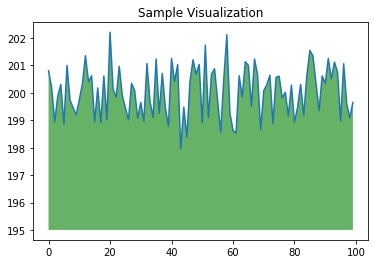
\includegraphics[width=0.8\textwidth]{chapter_1/figures/pythongraph.jpg}
    \caption{Graphical output of the PYTHON program}
    \label{fig:pythongraph}
\end{figure}

Let us analyse this program. First, its job is to make a plot of some random numbers. It probably isn't important exactly how long the code takes to produce this plot, as long as it isn't so long that it could have been done more efficiently without the computer. It also probably isn't critical that the program takes the same amount of time to produce this output every time it is run. 

The program makes use of some imported packages \texttt{numpy} and \texttt{matplotlib}, for mathematical functions and graphical output respectively.
It is somebody else's problem to implement these library functions. The \texttt{matplotlib} plotting function will only work if the computer has a way of outputting graphics. When I ran this code, the graphics appeared in my web browser, but this was because I was using Jupyter notebook; other python environments would have put the graphics in a separate window. 

Other observations about the program might seem obvious, but perhaps only because you have always taken them for granted. First, the program executes by default from top to bottom. Occasionally, there is a command that causes the code to go into a loop, so for example when the values of \texttt{ys} are generated, the
command \texttt{randn} generates 100 random numbers, so this random number 
generator loops around and runs 100 times before the program moves to the next
line of code. Similarly for the next line, which generates 100 values of \texttt{x}. All high-level programming languages feature loops, which cause code to execute multiple times. Another high-level programming concept is a conditional, meaning code that executes under some condition, but not if that condition is not satisifed. Loops and conditionals are so ubiquitous that you take it for granted that programs will utilise them. For that matter, you also take it for granted that code will execute from top to bottom.

Other things you might take for granted are particular to PYTHON. Notice how variables such as \texttt{x}, \texttt{ys} and \texttt{facecolor} represent data of different types, and that the type of data they represent is set automatically by PYTHON when the variables are defined. You don't generally have to declare what type of data a particular variable is going to be set to before that variable is used, PYTHON figures things out on the fly. In this respect, PYTHON differs from other high level languages like C or C++; in those languages you need to DECLARE a variable, including its data type, before you use it. You might think about whether this characteristic of figuring out variable types when they are first used is always a good thing, or whether perhaps it might occasionally cause problems.

The structure of high level computer languages generally comes about from them being intended for programming computers of a particular type. For example, most computers revolve around a very small number of processor cores which do all the calculations. Of course on a modern computer this may be less true than it used to be; there are often many cores on a CPU, and that doesn't include the GPU chip, where there are hundreds or thousands of cores that are more special purpose. In general, however, the architecture we imagine in a computer is that of a processor doing all the calculations, and input data and commands being piped in to this processor in sequence, and output form the processor coming out, so to speak, of the other side.

However, things do not have to be this way. In a more general calculating circuit, you can imagine the input data feeding in to the circuit through multiple parallel paths into a variety of different elements that all do things to subsets of the data at once. Such a circuit could be vastly more efficient than the gridlock that occurs when everything has to be stuffed in to a small number of processor cores. However, there is a price to pay, which is that the calculations in all these elements must be coordinated with each other, so that the outputs of the elements may combined and fed into yet more elements so that more calculations can be done, but on the right numbers. This way of doing things is potentially far more powerful than a conventional single processing unit architecture, but the programming of such a machine is vastly more complex as well. And, consider, the arrangement of the calculating elements for a particular computation may also need to be optimised for the efficiency of that computation. For the next computation, you may want to arrange the circuit differently.

So, in this course, we will consider the construction of digital circuits that do calculations. These circuits are literally wires connecting very fundamental building blocks. Until the 1980s. digital circuits were assembled using literal physical wires or circuit boards, connecting these fundamental blocks together. If you wanted a new circuit, you had to build it out of hardware. In the 1980s, however, large scale integration of digitial hardware led to a more abstract way of doing things. You described the digital circuit that you wanted using a new type of language, a Hardware Description Language (HDL). By a wierd stroke of luck I programmed early circuits of this type, which were called PALs, or programmable arrays of logic, using an early HDL called ABEL, when I was doing work experience at school. I had no idea that I would wind up using it's direct descendent, called VHDL, a far more advanced hardware description language, in my physics research more than 35 years later. Life is strange sometimes. Anyway, the hardware description language literally permits you to build a digital machine. You are building hardware, using a language.

Having built the hardware, in simple cases, you just pipe the data in, and the desired output appears at the other end of your digital machine. This has two great advantages. First, it is extremely fast. There is no operating system or other environment to slow down the process. Second, often the calculation takes exactly the same amount of time every time it is executed. This makes this type of machine suitable for use in situations where the output of the calculation is used to control the state of something critical, like a physics experiment, where unexpected delays cause glitches which may cause the machine or experiment to stop working.

In more complex cases, your machine may grow to resemble a computer, and you may need to write more code, this time perhaps in a high level language, to program it. But because you have far more control over the architecture of your machine than yo do with an ordinary computer, you are empowered to make a far more interesting, useful and powerful calculation engine. I hope you will enjoy learning physical computing, as I have enjoyed it. It's physics, but not perhaps as you have experienced it before.

\section{Lab Number 1. Getting to know the Development Hardware}
\label{sec:exploring_our_hardware}

We will develop our hardware and software in an integrated development environment called Vivado/Vitis, and deploy to a development board. The development environment will be running on your loaned Lenovo ThinkPad i7 PC and the test hardware consists of a BASYS3 development board. These are connected together with a USB to micro-USB cable. 

The Lenovo ThinkPad runs Ubuntu, a dialect of the LINUX operating system, which is an example of the UNIX family of operating systems that has been around since the mid 1970s. The choice of LINUX rather than Windows is for many reasons, but here I highlight one of them. Microsoft has a habit of inducing Windows to install updates at random times. Experience taught us that too often students were sitting in the lab waiting for a windows update to complete, and there was no obvious way to stop this happening. In UNIX, updates are very much under the control of the administrator of the system. In the case of your laptops this is Mitch, and we only update in the off-season! There are other reasons but this is the main one.

The PCs are quite nice and in particular quite fast because they have several intel i7 processor cores, and the software we are running to program the BASYS3 boards can make use of these in parallel. They do have some annoyances. The main one is the rather small screen. If at home you have an HDMI monitor and cable, then you can use an ordinary HDMI cable to connect the laptop to an external screen, which makes using the computers more comfortable. You can also plug in your own mouse via USB. The other annoyance is the ‘PgUp’ and ‘PgDn’ (page up and page down) buttons being located right next to the cluster of arrow buttons on the keyboard, which means that sometimes you find yourself taking forays into bits of your code you didn’t intend to visit. There is nothing that can be done about this; I only flag it in case you don’t understand what is happening, and advise you to be conscious of exactly where your finger is when trying to use the arrow keys. You can use a USB mouse with the laptops - just plug it in and it should start working. One with a 'wheel' on it can be particularly useful for scrolling up and down code and documents, like this book.

The BASYS3 boards are designed for teaching purposes are are therefore easy to use relative to other development boards we have tried. However, the hardware on these boards is quite cheap, and occasionally fails. Please do not leave the connecting cable plugged in to the USB port on the board when you put it in your bag to carry it around! This is a great way to destroy the rather fragile USB connector on the board. The other failure point is the 16 LEDs and switches along the bottom edge of the board, below the BASYS3 logo. The switches wear out quite quickly, and the LEDs (rather surprisingly) also fail quite often. In todays project we will check all the switches and LEDs on your boards.

You will all be learning to use LINUX, which many of you will never have met. This should not be a handicap on the course. An important difference between LINUX and Windows is that in LINUX the command line interface, accessed by opening the terminal program, is a very powerful environment. Windows users mostly abandoned the DOS prompt and direct issue of commands to the operating system many years ago, although amongst engineers, scientists and developers DOS still does get used, in spite of its many shortcomings. In LINUX it is common to make use of commands issued directly into a terminal for tasks like creating directories, moving files, and communicating with other machines on the internet using various communication protocols (ssh, sftp, git and other things that we shall learn about). You’ll find yourself using the terminal window to get things done. This is a useful transferable skill into many lines of work and post degree research.

The laptops have all been set up with the same environment and software. You will find that you do not have permission to install your own software on the system or make major changes to the way your computer is set up. It is not in your interest to make major changes to the system -  for example trying to repartition the disk and install a windows operating system on a separate partition. We therefore make a rule against attempting such hacks, and Mitch will not be happy, and will tell me (and I will be even less happy) if it becomes clear that somebody has broken this rule. 

One final point. This is a course that teaches practical skills. As with other practical skills – riding a bike, playing a musical instrument, etc, real facility comes with practice. The labs give you a total of about 33 hours of time officially dedicated to this. However, because I am lending you the hardware, you can also practice outside labs, and are strongly encouraged to do so. In about 5 years of teaching the course, several of our students have used skills gained on the course to get very good jobs in companies. I am very much hoping to have one of them talk to you all about their experience in industry using things that we taught on this course. The course is largely what you make of it. If you work hard, you are gaining some genuinely useful skills for your CV and future career, if that is what you decide you want.

\section{Brief Tour of the Laptop}
\label{sec:brieftour}

The first job is to turn on the laptop, and log in under the physics user. Your username will remain ‘physics’ for the duration of the course.

The first job is to connect the laptop to the campus wifi. It will not connect by default – Mitch has wiped the hard drive and it is essentially equivalent to a fresh-out-of-the-box system. 

With the exception of the very first instruction, the instructions below are identical to the University’s seen at \url{https://students.sheffield.ac.uk/it-services/wireless/connect#linux}. These are to be followed with one exception. The root certificate download can be found on the laptop already at \\ \texttt{/etc/ssl/certs/QuoVadisOVRootCertificate.crt} :-

\begin{enumerate}
\item{Click on the downwards arrow in the top right hand corner of the desktop and select `Wifi Not Connected' then `Select Network', then select eduroam, then press the `Connect' button at the bottom of the selection window.}
\item{{\it NOTE - you do not have to follow this instruction because the file is already on your machine at the path above.} Download the QuoVadisOVRootCertificate.crt certificate to your machine from \\
\url{https://www.sheffield.ac.uk/polopoly_fs/1.950471!/file/QuoVadisOVRootCertificate.crt}.\\
}
\item{When in range of eduroam click on it to enter settings.}
\item{Use the following settings:
\begin{itemize}
\item{Wireless Security: WPA2 Enterprise}
\item{Authentication: PEAP}
\item{CA Certificate: Browse to where you saved the certificate and select}
\item{Inner Authentication: MSCHAPv2}
\item{Username: Your UoS username followed by @sheffield.ac.uk}
\item{Password: Your UoS password}
\end{itemize}
You should then be able to connect to eduroam}
\end{enumerate}

Figure \ref{fig:emptyscreen} shows the Ubuntu window manager you should see when you have logged in. Down the left hand side there are a set of icons in a toolbar that run different pieces of software. Yours are not quite the same as mine as I have added a few extras. On your machines, there are seven that will prove useful during the course. By hovering with your mouse pointer over the icon you can see what these applications are. Locate the following applications:

\begin{enumerate}
    \item Firefox Web Browser
    \item Files
    \item Terminal
    \item Serial port terminal
    \item Vivado 2019.2
    \item Xilinx Vitis IDE 2019.2
    \item Documentation Navigator
\end{enumerate}

\begin{figure}
    \centering
    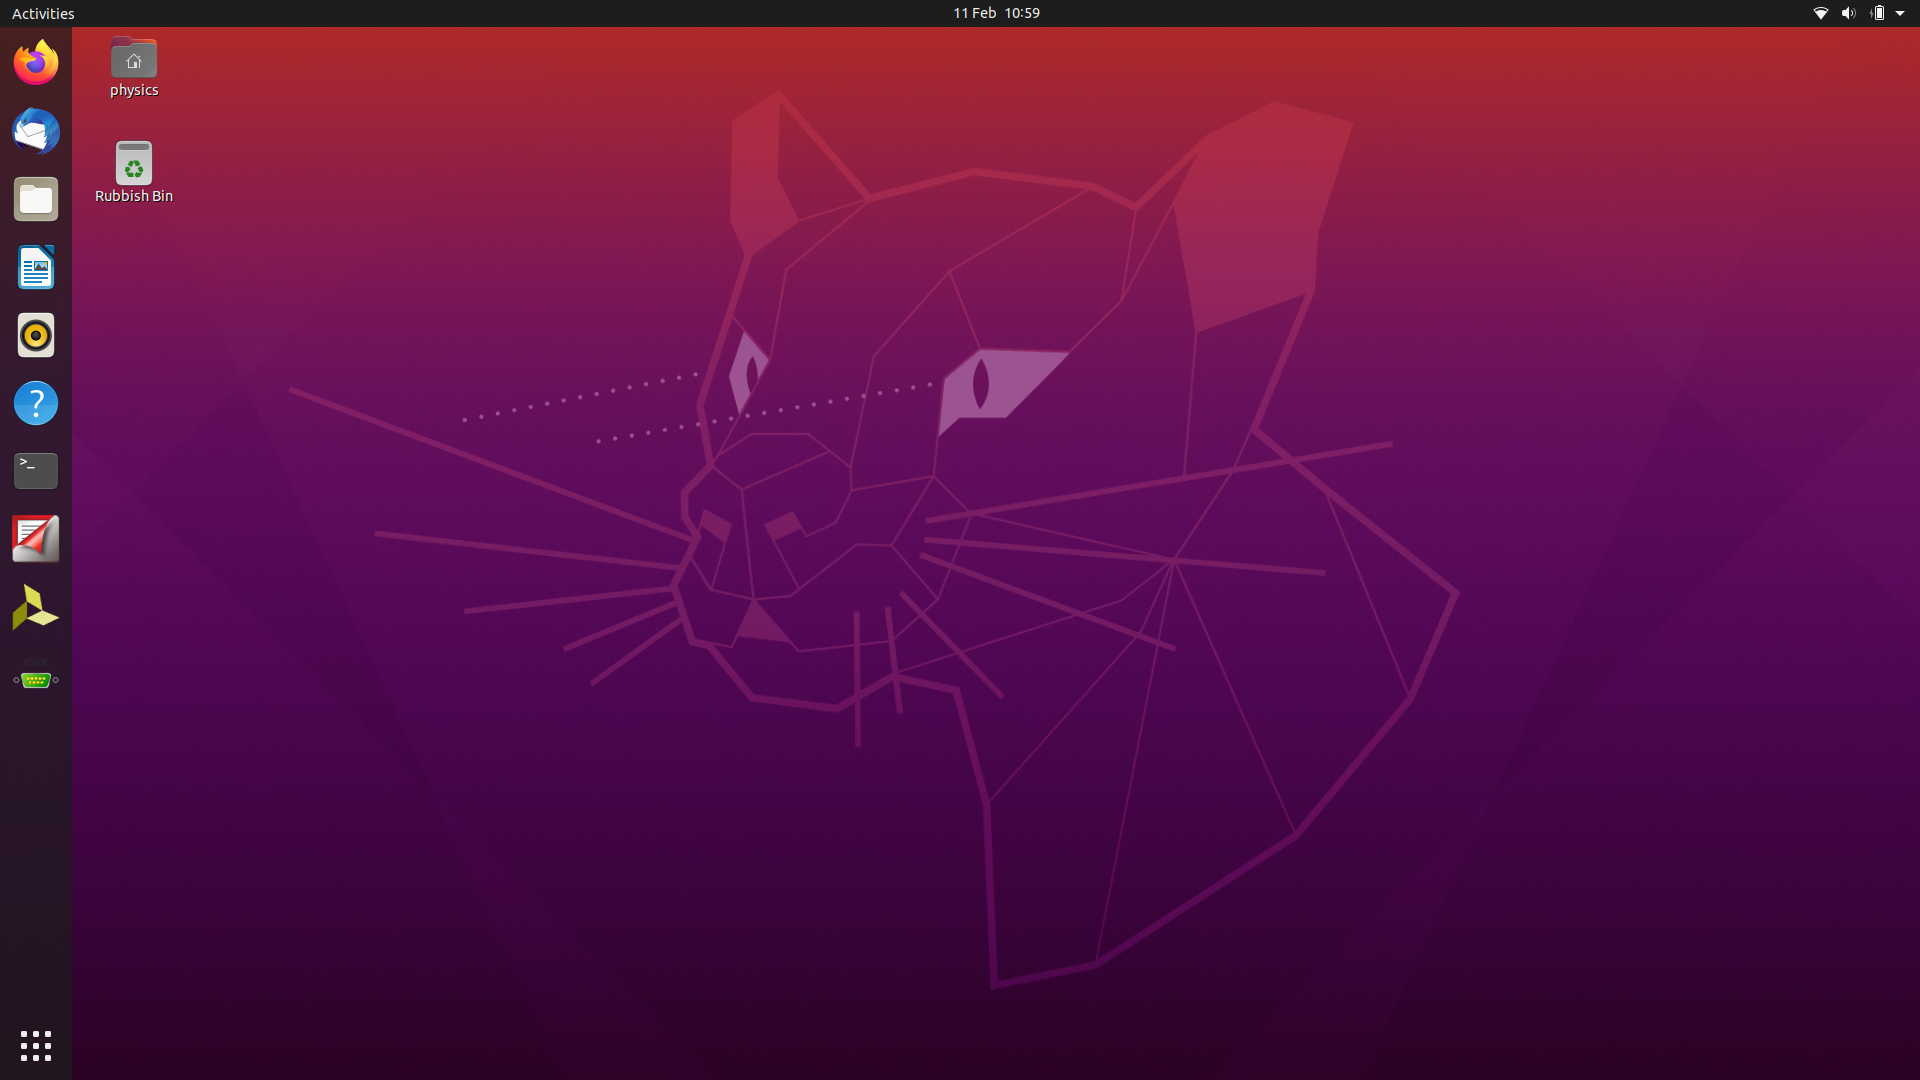
\includegraphics[width=\textwidth]{figures/blank_ubuntu_screen.png}
    \caption{A blank screen upon logging in as physics to Ubuntu}
    \label{fig:emptyscreen}
\end{figure}

You can single-left-click on any of these items to run the corresponding applications. If you run something and want to stop, just as in Windows, use the red 'x' in the top right hand corner of the window. Most windows can be resized by dragging on the corners, minimised by clicking on the underscore also in the top right corner, and expanded to full-screen mode by clicking on the rectangle in the same place. If you minimise a window belonging to one of the sidebar applications, it can be recovered by clicking again on the icon. You can also re-open a minimised icon by clicking on 'Activities' in the top left hand corner. The full set of installed applications can be seen by clicking on `nine dots' icon in the lower left corner. You can drag across the mouse pad to go up and down the full set of icons. Clicking on it again takes you back. If you are alone and want some background music or talk, the 'RythmnBox' application plays podcasts. 

The two icons in the top left of the main window are short-cuts to the Files application running on your home directory and the contents of the rubbish bin

Firefox should need no explanation. The `Files' application is like the Windows file manager, and it allows you to navigate through the hierachy of folders on the Ubuntu machine. If you right click on a file you are given an option to move to the recycle bin, just as in Windows. In fact, Ubuntu is trying to emulate the Windows operating system. The big difference between Linux and Windows is the use of the Terminal application. Windows has the DOS prompt, but DOS is so arcane that few but the brave use it very much. In Linux the Terminal 'shell' is the BASH shell, which has quite a lot of functionality and is quite sophisticated. However, you shouldn't actually need to learn too much UNIX/Linux to do this course. If you are interested, there are lots of tutorials on line in learning the BASH shell in UNIX/Linux. The serial port terminal will be useful later in the course when we are communicating with microprocessor cores on the BASYS3 board. Vivado and Vitis are the two graphical user interfaces that we will use to develop our applications. We will spend most of our time using Vivado and Vitis.

Before you can use Firefox you will need to connect your laptop to a wireless network. The icon to do this is in the top right hand corner of the screen and looks like a segment of fruit. If you click on this icon it will show you a list of available wireless networks - you should check and see that there is one that you can log in to. After logging in, the segment will be partially filled in, indicating the quality of your connection.

You should be able to use Firefox to log on to MUSE and from there with the google mail tool and Blackboard you should be able to use your laptop to take part in the lab projects without need for your own personal devices. The camera built in to the laptop and the built in microphone both work with blackboard and we will need to communicate with each other freely to make a success of the course, within the limits imposed by bandwidth.

To shut the laptop down, the small downwards arrow in the very top right pulls down a menu from which you can select the Power Off/Log Out option, and there you can do all the usual things - turn off, restart, log out, etc. In these things Ubuntu again behaves much like other popular operating systems.

There are also several other equipment items. These are, all told
\begin{enumerate}
    \item Cardboard box and packing material (please preserve in good condition)
    \item Laptop with power supply (two connected cables)
    \item Gel filled protective laptop case
    \item USB to micro-usb adaptor cable
    \item Basys3 FPGA development board
    \item PMODDAC2 two channel digital-to-analog converter (DAC) - this is small!
    \item some cables
    \item a crystal earpiece
\end{enumerate}

Obviously try not to lose anything and tell me if you do, or if anything gets broken. Try NEVER to keep drinks anywhere they can spill on the laptop. Especially on the table directly next to them. Think of them as lab equipment. You wouldn't drink in a lab, so don't keep drinks in the vicinity of this machinery.

One final thing about the laptops. If you want to dump the whole screen to a picture file, then at any time you can just press the PrtScr button which is on your keyboard two keys to the right of the space bar, and a `.png' format bitmap of the entire screen is written to the Pictures subfolder of your home directory. Try this, and then use the Files application to go to this directory, double clicking on the icon to view it. If you just want to print one window, make sure this window is selected, then hold down the Alt key and again press PrtScr (Alt-PrtScr), and a `.png' file just of the highlighted window is put in the same place. This could be useful if something isn't working right and you want to send myself or Mitch graphics that are useful in explaining your problem.

\section{Logic Gates}
\label{sec:logicgates}

We start our physical computing course where all beginners courses on digital circuits begin, with logic gates.
A logic gate is an abstract operation having a single digital output and one or more digital inputs. There are seven
logic gates that you will see on schematics. The simplest of them is a NOT gate, or inverter, mentioned in the preface,
whose output is $1$ when its single input is $0$, and $0$ when the input is $1$. The next simplest gates each have two inputs. The two input AND gate has output $1$ only when both its inputs are $1$, the two input OR gate has output $1$ when either or both of its inputs are $1$, and the two input XOR (exclusive or) gate has output $1$ when either one, but not both, of its inputs are $1$. That's four so far. The other three gates consist of the AND, OR and XOR gates with an inverter on the output, forming the NAND, NOR and XNOR gates. The six two-input gates generalise to more than two inputs. For example, a 3 input XOR gate has output $1$ when any one, but not more than one, of its inputs is $1$.

An alternative to these written descriptions of functionality is to tabulate the outputs for each possible combination of inputs. Such tables are called truth tables. The truth tables for the four gates NOT, AND, OR and XOR are shown in Figure \ref{fig:logic_gates_figure}
along with the symbols representing the gates. The figure caption tells you how to draw the other three gates NAND, NOR and XNOR. 

\begin{figure}[t]
\centering
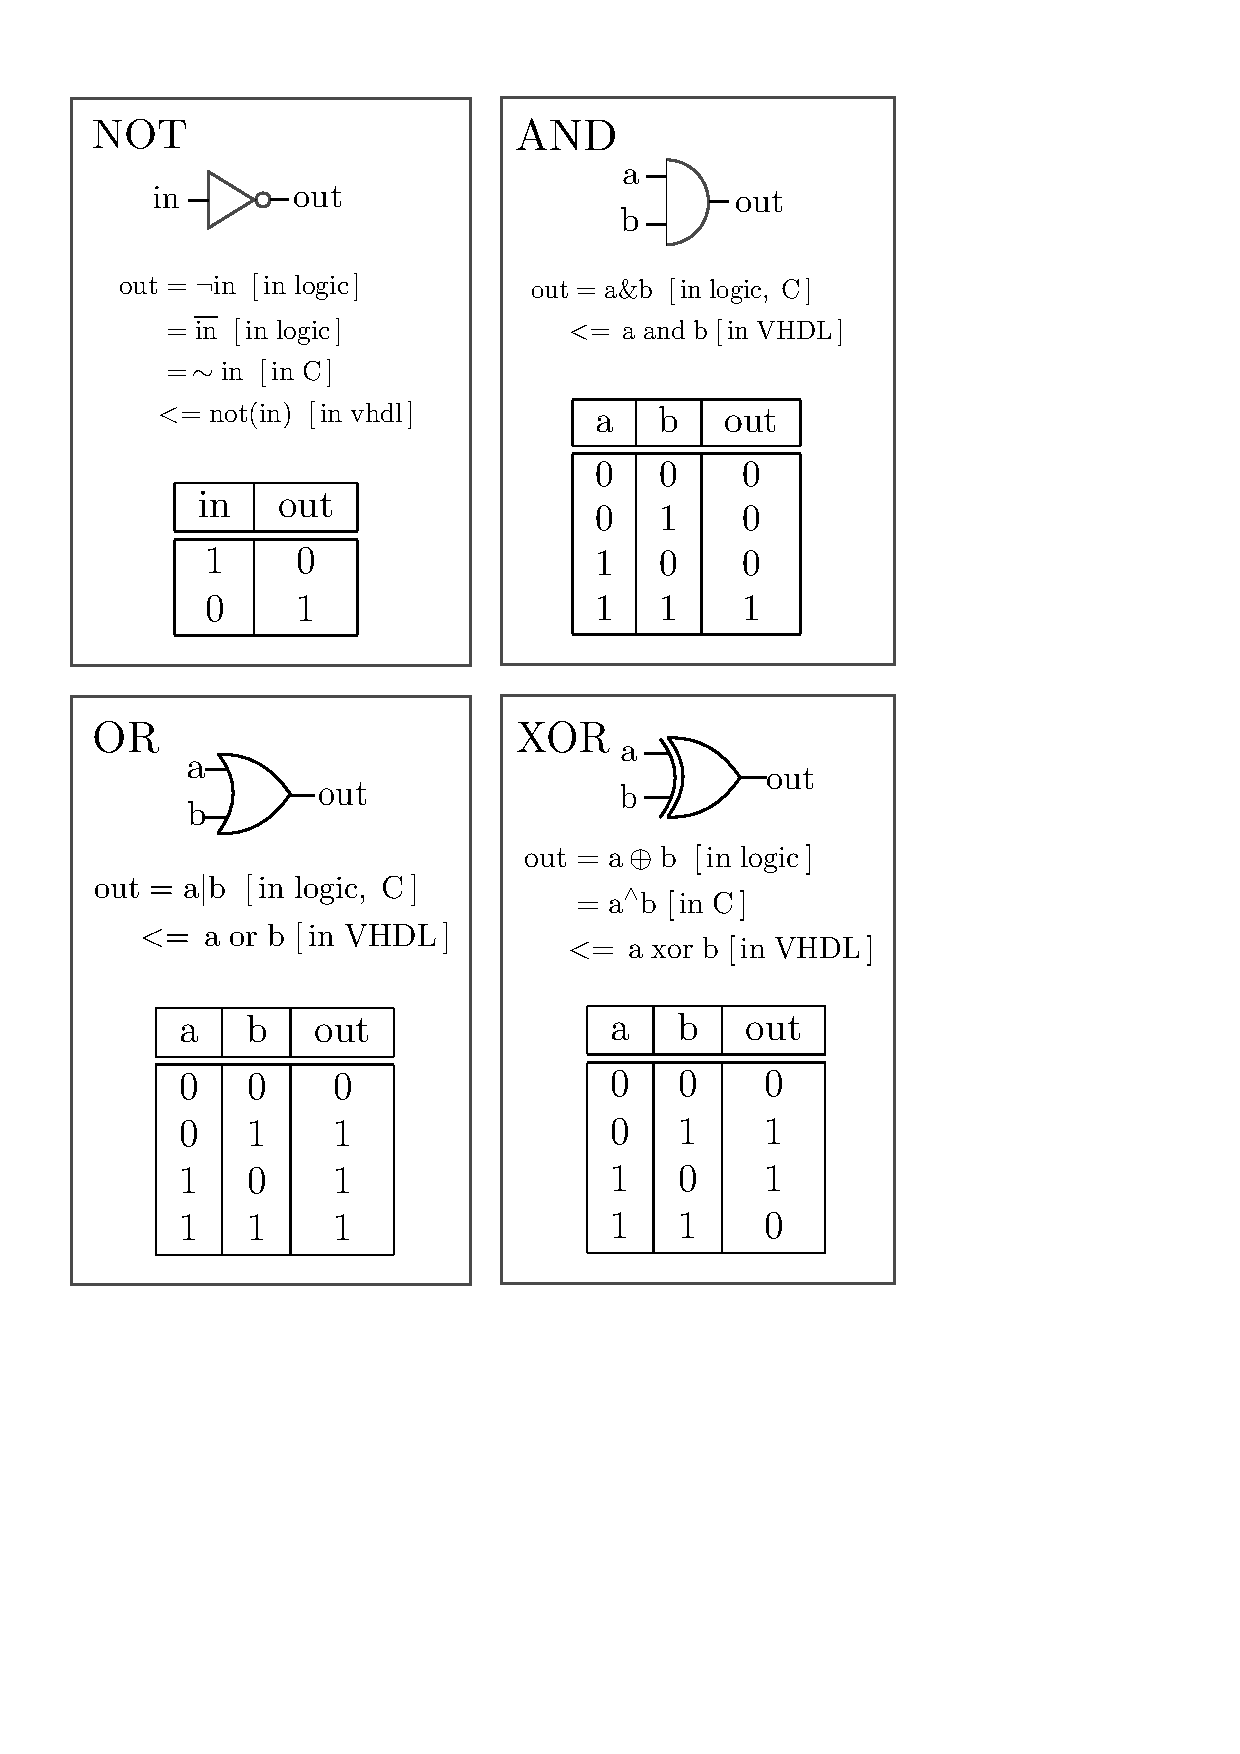
\includegraphics[width=0.5\textwidth]{figures/logic_gates_figure.pdf}
\caption{\label{fig:logic_gates_figure} Truth tables and symbols for four of the seven logic gates commonly encountered. The other three, NAND, NOR and XNOR are obtained by adding a not at the output of AND, OR and XOR, respectively. The symbols are the same as for AND, OR and XOR except for the addition of a small circle like that on the right side of the NOT gate. Sometimes you will also see a small circle on one of the input leads before the gate body. For example, if this circle before the body of the AND gate appears on the b input, it means `a and not b.'}
\end{figure}

\section{De Morgan's Laws}
\label{sec:demorgan}

It turns out that you can build AND gates out of OR gates and NOT gates, or OR gates out of AND gates and NOT gates, as a consequence of a useful piece of maths that comes from the theory of sets, called De Morgan's laws. In the theory of sets, if $A$ and $B$ are each sets, then $A\cap B$ is called the intersection of $A$ and $B$, and means all the elements that are in both set A and set B, and $A\cup B$ is called the union of $A$ and $B$ and means all the elements that are set A or set B. So there is a direct correspondence between the logical $\rm AND$ and the intersection, and between the logical $\rm OR$ and the union. What about $\rm NOT$? In set theory the symbol for all the elements not in set $A$ is the complement of $A$, or $\overline{A}$. There are two De Morgan's Laws, and both can be stated either in set notation or in logic notation. The logical statements are

\begin{figure}[h!]
    \centering
    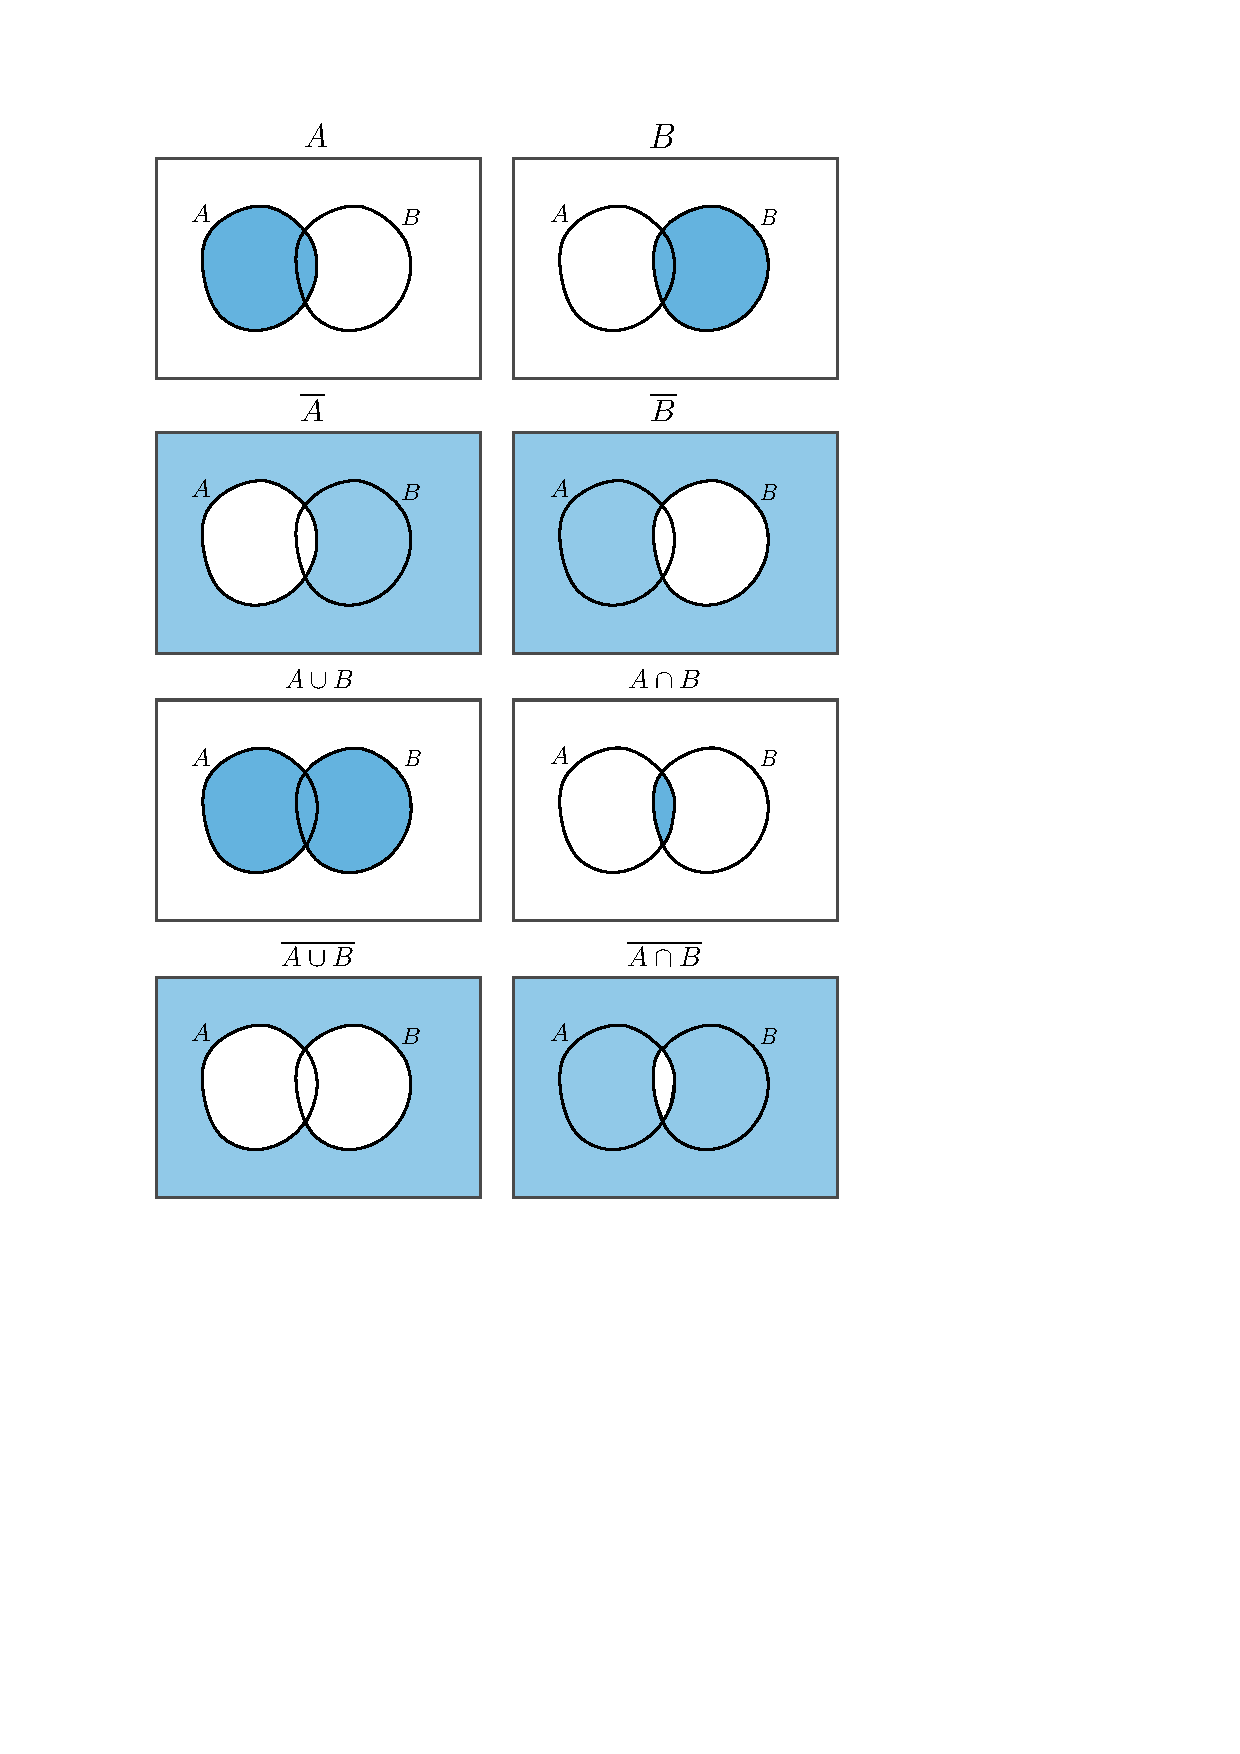
\includegraphics[width=0.45\textwidth]{figures/venn_diagram_figure.pdf}
    \caption{\label{fig:venn_diagram_figure} Venn diagrams illustrating De Morgan's laws.}
\end{figure}

\begin{align}
\neg(a\&b) &= \neg a | \neg b
\label{eq:demorganone} \\
\neg(a|b)&=\neg a \& \neg b.
\label{eq:demorgantwo} \\
\nonumber
\end{align}
In words, Equation \ref{eq:demorganone} states that not(a and b) is the same as (not a) or (not b), and Equation \ref{eq:demorgantwo} states that not(a or b) is the same thing as (not a) and (not b). The same two laws can be stated in set notation as
\begin{align}
    \overline{A\cap B}&=\overline{A}\cup\overline{B}
    \label{eq:demorganoneset} \\
    \overline{A\cup B}&=\overline{A}\cap\overline{B}.
    \label{eq:demorgantwoset} \\ \nonumber
\end{align}
If you like Venn diagrams, you can prove De Morgan's Laws with them. This is done in Figure \ref{fig:venn_diagram_figure}. The rectangle represents all objects in some space, everything inside the left hand ellipse is in set A, and everything inside the right hand ellipse is in set B. The complements of $A$ and $B$ are shown in the second row. The union and intersection of $A$ and $B$ are in the third row. The fourth row shows the complements of the union and the intersection of $A$ and $B$. The union of $\overline{A}$ and $\overline{B}$ is the areas that are blue in either of the diagrams in the second row. This is everything except the thin white sliver common between both $A$ and $B$, in other words it is the complement of the intersection of $A$ and $B$. This proves De Morgan's first law, Equations \ref{eq:demorganone} and \ref{eq:demorganoneset}. The intersection of $\overline{A}$ and $\overline{B}$ is the areas that are blue in both of the diagrams in the second row. This is everything that isn't in either of the white ellipses of $A$ or $B$, in other words it is the complement of the union of $A$ and $B$. This proves De Morgan's second law, Equations \ref{eq:demorgantwo} and \ref{eq:demorgantwoset}.

De Morgan's laws simplify the job of chip designers since essentially all of the logic gate elements on a chip may be fabricated out of either OR gates or AND gates, plus inverters. Figure \ref{fig:de_morgan_logic} is a third statement of De Morgan's laws in terms of the symbols for the gates themselves.

\begin{figure}[htbp]
    \centering
    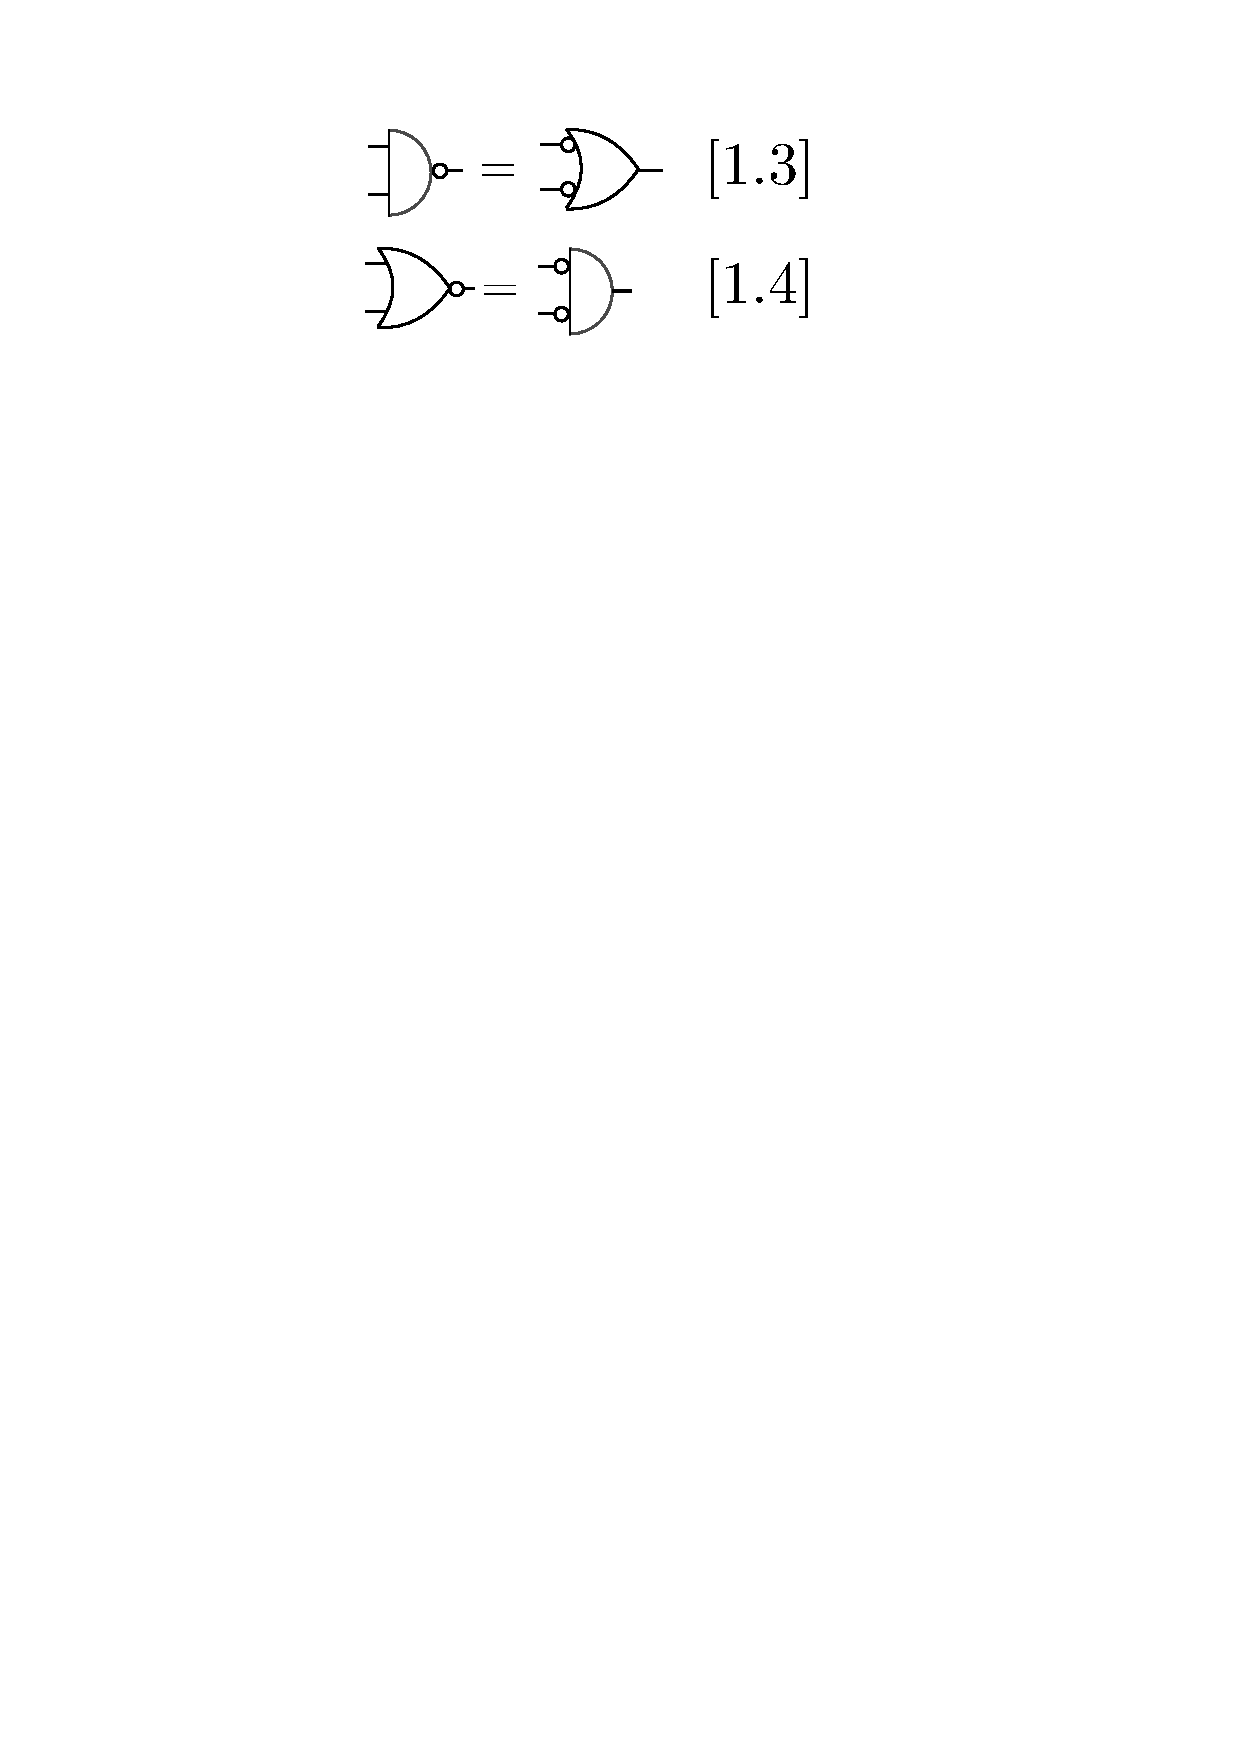
\includegraphics[width=0.2\textwidth]{figures/de_morgan_logic.pdf}
    \caption{\label{fig:de_morgan_logic} De Morgan's laws in terms of the equivalence between different types of logic gate.}
\end{figure}

\section{Parallel Buses}
\label{sec:parallel_buses}

We aren't going to get very far if we only ever deal with one bit at a time. The simplest way to streamline manipulations of multiple bits is to perform the same operation on many bits in parallel. A collection of bits in parallel is called a bus, and the number of bits in the bus is called the bus width. Frequently buses consist of 8, 16 or 32 bits in parallel. There are other kinds of buses other than parallel, and we will discuss some of these presently, but for now just imagine an assembly of signals in a set of wires. Buses are ordered. In other words, the position of a particular bit of a bus is well defined. Usually we think of a bus as an ordered set of bits from left to right, with the rightmost bit called the least significant bit, or LSB, and the leftmost bit called the most significant bit, or MSB. This is in preparation for use of parallel buses to represent integers, which we will discuss in Section \ref{sec:logic_and_integers}. 

The logic operations defined in Section \ref{sec:logicgates} were so far discussed as operating on a single bit, but they can also operate on buses containing many bits, so long as each input and output has the same bus width. Used in this way, the logic operations NOT ($\neg$), AND ($\&$), OR ($|$), XOR ($\oplus)$, NAND ($\neg\&$), NOR ($\neg|$) and XNOR ($\neg\oplus$) are examples of `bitwise' operations, in that they operate on each bit separately and do the same thing to all the bits. So, for example,
\begin{align}
    \neg\,B00010000&=B11101111
    \label{eq:first_bus_operation}
\end{align}
 and
\begin{align}
   B10101010\,|\,B00010000\,&=\,B10111010.
   \label{eq:second_bus_operation}
\end{align}
 Here I have used the notation of a leading $B$ to mean that the sequence of digits following represents a bus of bits - just a way of expressing whether the bits in a bus are high or low, $1$ or $0$, or equivalently true or false.
 
 There are other binary operations that can only meaningfully act on parallel buses of bits. Bit shifting operations, in particular, involve shifting the values in all the bits in a bus to the left (in the direction of the most significant bit) or to the right (in the direction of the least significant bit). As a consequence, either the rightmost or the leftmost bit falls off the end of the bus and is lost, and a gap appears at the other end. In a logical bit-shift operation, the gap is filled with a zero. In an arithmetic bit shift, the gap is filled with a copy of the value in the bit that must moved along to create the gap. Finally, you could possibly place the value in the bit that fell off the other end of the bus in this position. All three types of bitshift operations can sometimes be needed. Where the bus is representing logical rather than arithmetical data, logical bit shifting is the most common. An exercise in Appendix \ref{sec:logic_in_vhdl} will show you how to execute logical bit shifts on buses representing logical data in the hardware description language VHDL.
 
 The use of binary operations to simplify and speed up computer code is an interesting subject. There is a nice book by Warren \cite{Warren:10.5555/2462741} where you can read about logical consequences of De Morgan's laws and mathematical tricks involving bitwise logic operations combined with bit shifts, particularly in Chapters 1 and 2, which I will make available to you on Collaborate.

\section{Logic and Integer Arithmetic}
\label{sec:logic_and_integers}

\subsection{Logic and the Foundations of Mathematics}
\label{sec:logicandmathsfoundations}

De Morgan's laws are an example of the connection between the theory of sets and logic. This is natural because both sets and logic are closely connected to the foundations of mathematics. The drive to build a logical foundation for mathematics was an area of intense activity at the turn of the 20th century. The famous series of books, Principia Mathematica, by Russell and Whitehead \cite{Whitehead:268025}, an attempt to build a consistent and complete logical foundation for mathematics, famously collided with the philosophy of Kurt G\"odel who proved that the task is impossible. Modern formulations of axiomatic set theory, or the logical foundations of mathematics, are based on Zermelo-Fraenkel set theory, and it is in this context that modern developments in the logical foundation of mathematics are usually discussed. The subject of the logical foundations of mathematics is fascinating. If you are interested, and there are many popular books on the subject which will stretch your mind, especially if you try and do the puzzles \cite{Hofstadter:99665,Smullyan} !

Fortunately we do not need to construct a complete logical basis for mathematics, only to work out some ways of using logic gates to do simple arithmetic, which is much easier. Nonetheless, we shall quickly discover that in using logic to do mathematics you have to be careful to avoid encountering difficulties. These difficulties shall be discussed in Chapter \ref{sec:registers}.

\subsection{Binary Representation of Positive Integers}
\label{sec:postiveintegers}

Let us first consider representation of integers. Bits naturally lead to the use of binary numbers to represent integers. Any sensible representation will have the integer zero represented by any number of $0$s, and the integer one represented by a single $1$. If the integers are all positive or zero, then all we need is ordinary binary numbers, so the numbers 0 to 15 can be represented by three binary digits. In ascending order, $B0000$, $B0001$, $B0010$, $B0011$ $B0100$, $B0101$, $B0110$, $B0111$, $B1000$, $B1000$, $B1001$, $B1010$, $B1011$ $B1100$, $B1101$, $B1110$, $B1111$. If we want to represent any larger number than 15, we will need more bits in our binary representation than four. The largest unsigned integer representable using an $N$ bit parallel bus is $2^N-1$.

\subsection{Hexadecimal Notation}
\label{sec:hexadecimal}

I am already getting tired of writing all those zeros and ones, and in digital signal processing it is common to represent collections of binary numbers using hexadecimal, or base 16. Because people commonly have ten figures, we have developed naturallly to have symbols for each of the counting numbers between 0 and 9, and think of larger numbers as groups of 10, or groups of 100, and so on. However, suppose we had actually had 16 fingers! We would then have naturally developed separate symbols for the first 16 integers 0 to 15 that are also each representable by four binary bits. Table \ref{tab:hexadecimal} shows the first 16 numbers from the set of positive integers and zero, together with their decimal and hexadecimal representations.

\begin{table}[hbt]
    \centering
    \begin{tabular}{|c|c|c|}
    \hline
         decimal & binary & hexadecimal \\
         \hline\hline
         0 & B0000 & 0x0 \\
         1 & B0001 & 0x1 \\
         2 & B0010 & 0x2 \\
         3 & B0011 & 0x3 \\
         4 & B0100 & 0x4 \\
         5 & B0101 & 0x5 \\
         6 & B0110 & 0x6 \\
         7 & B0111 & 0x7 \\
         8 & B1000 & 0x8 \\
         9 & B1001 & 0x9 \\
         10 & B1010 & 0xa \\
         11 & B1011 & 0xb \\
         12 & B1100 & 0xc \\
         13 & B1101 & 0xd \\
         14 & B1110 & 0xe \\
         15 & B1111 & 0xf \\
        \hline
    \end{tabular}
    \caption{Decimal, binary and hexadecimal representation of zero and the first fifteen positive integers.}
    \label{tab:hexadecimal}
\end{table}

The hexadecimal notation is extensible to numbers represented by many more bits. For example, on computers integers are commonly represented as 32 bit binary numbers, so that the unsigned integer 1 would be represented as $\rm B00000000000000000000000000000001$. In hexadecimal this is $\rm 0x00000001$, which is still a lot of leading zeros, but you can see how the reduction in the number of symbols by a factor of four when using hexadecimal notation instead of binary is attractive.

\subsection{Binary Counters and Oscillators}
\label{sec:oscillators}

While we are looking at this table, it makes obvious another useful feature of binary numbers, and that is the behaviour of the binary digits. Scan down the column of binary numbers and look only at the least significant bit (LSB). Notice that as the count proceeds, the least significant bit oscillates back and forth between $0$ and $1$ with a period of two counting numbers. Now look at the second-least significant bit. This bit also oscillates back and forth between zero and one, but the period of this oscillation is four counts. The third least significant bit also oscillates periodically with a period of 8 counts, and the most significant bit (MSB) has a period of the full 16 counts. This means that if we can cause a bus to count upwards from zero, each subsequent bit can serve as an oscillator with a period of twice that of the previous bit. It turns out to be very useful indeed to be able to make oscillators with different periods in digital devices, and we shall see the power of this in Chapter \ref{sec:registers}.

\subsection{Overflows in Binary Arithmetic}
\label{sec:overflows}

We have already realised that we need more than four bits to represent a positive binary number greater than 15. What is the convention for dealing with overflows? What happens when you add 1 to 0xf ? We will operate with the following convention, following digital signal processing conventions: {\it overflows are disregarded}. If you require more bits than you have designed into your system to get the right answer, it's just tough - you should have used more bits. While this might sound harsh, in fact the convention that overflows are ignored is very useful indeed.

The first reason for this is to do with counters. As alluded to before, if we count up in binary, each successively more significant bit behaves like an oscillator with half the period of the bit to the right. What about the most significant bit? What does it do? It starts out as 0, then half way to the maximum capacity of the bus, it switches to 1. What happens when it reaches full capacity? This is when all the bits are $1$. The next number in the sequence, {\it ignoring the overflow} is all zeros. In other words, the counter just resets to zero, and then keeps counting. A counter that starts at zero, then gets to the maximum number that can be represented with the number of bits, then resets to zero automatically and starts again, is very useful indeed!

There's another very useful application of ignoring overflows. It means that a binary number of N bits containing all 1s is adjacent in the sequence of binary numbers to a binary number containing all 0s. This comes in very handy when representing negative integers with a system called {\it twos complement} which we will discuss in the next section.

To summarise this section, in a binary representation of numbers, overflows are ignored. If you have 4 bits, then all numbers are represented using 4 bits, and if you end up running off the end, you neglect any overflows and instead your sequence wraps around back to the other end.

\section{Lab Exercise 2 - Logic in VHDL}
\label{sec:appendix_2}

\subsection{Creating a new Vivado project}
\label{sec:create_new_vivado_project}

VHDL is a hardware description language for expressing the abstract functionality of digital circuits. VHDL can be compiled into an actual wiring diagram for a specific hardware device, which in this course will be a field programmable gate array, or FPGA. The FPGA we will be using in this course is from the Artix7 series made by Xilinx. Specifically the part number of the Artix7 FPGA on your BASYS3 boards is \texttt{\bf xc7a35tcpg236-1}. This is a part number that you will need every week in the lab. 

The compiler that tries to turn your VHDL code into a hardware specification is actually a command line tool, but like many such tools it is usually used by way of a graphical user interface, sometimes called a software development kit (SDK). SDKs are all over the engineering world. In this course we will be using two SDKs, Vivado and Vitis. Vivado is the SDK for building the hardware, and when the hardware incorporates a microprocessor, Vitis is the SDK that we will use to program that microprocessor in the C language.

A few practical details. You may have noticed that the chapters of the book correspond to the material taught in lectures, and the appendices correspond to the labs. This is deliberate. The lecture material I consider to be implementation independent; it would be the same if we were using a different HDL made by a different company for different chips, or a different SDK. The appendices are specific to our hardware. The idea is that I may have to re-write the appendices many times, but I am hoping not to have to do too much rewriting of the chapter materials.

So, let's get started. For our first project we will build hardware that allows us to check that all the switches and LEDs on the BASYS3 board are working. There are two reasons for doing this. First, they might not be. The components of the BASYS3 are fairly cheap and it is not uncommon for the switches in particular to wear out and stop working. The second reason is that this is one of the simplest projects we can do, so it is a good one to start with.

You will need to have read Appendix \ref{sec:our_hardware} before starting these instructions. Start up Vivado using the left hand tool shortcut. After some delay the window shown in Figure \ref{fig:vivado_startup} will appear. Note that some people become impatient and click the icon twice in which case two copies of Vivado will open. Just close one of them if this happens and use the other one.

\begin{figure}[htbp]
    \centering
    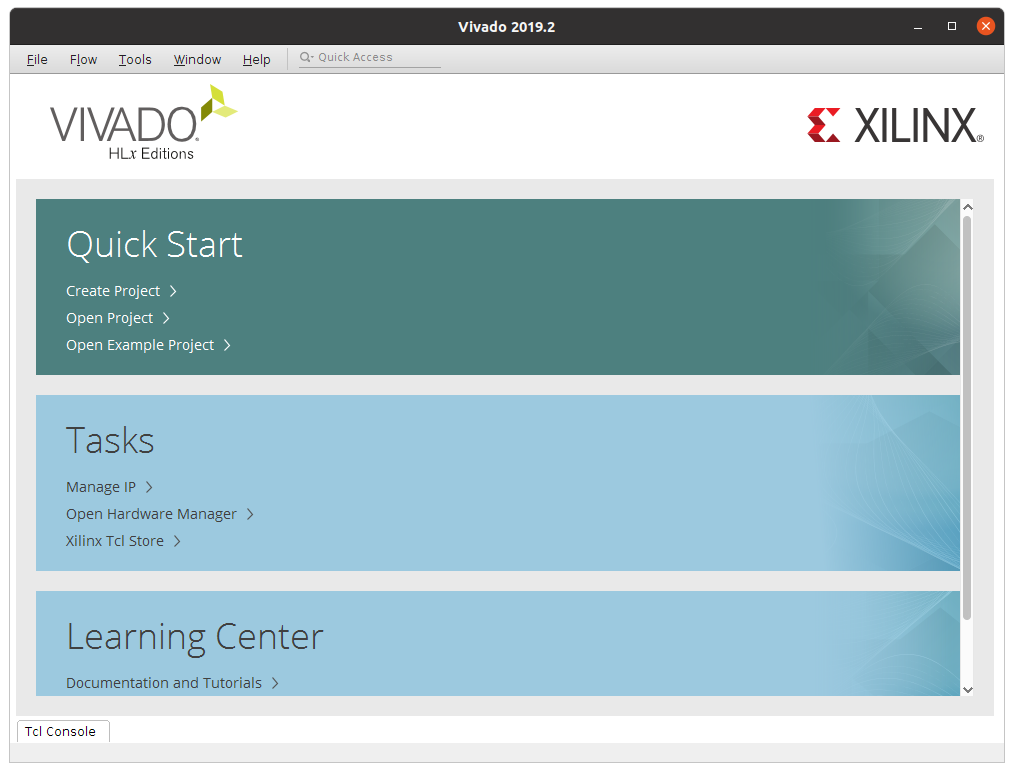
\includegraphics[width=0.8\textwidth]{figures/vivado_startup.png}
    \caption{Startup screen for the Vivado software development kit}
    \label{fig:vivado_startup}
\end{figure}

You'll want to create a project, so left-click (henceforth whenever I ask you to click without specifying which button, I mean left-click) on `Create Project'. This brings up a subwindow that says `Create a New Vivado Project'. On the first page you are asked to give the project a name, and to specify its location. Let's call the project \texttt{check\_leds\_and\_switches}. It is an old habit of mine to use underscores instead of spaces in file and directory names. I recommend that you pick up this habit. Unix-like computers tend to place special meaning on whitespace characters like space, tab, etc and things can unexpectedly fail to work if you have files and folders that have spaces in their names. Change the project name by clicking in the box and typing the new name. For the project location, the default is your home directory but we don't want this directory to become too cluttered, so let us make a new place to keep our Vivado projects. Click on the small rectangle to the right of the Project location box, with three dots in it. This brings up a 'Choose project location' window, shown in Figure \ref{fig:choose_project_location}. 

\begin{figure}[htbp]
    \centering
    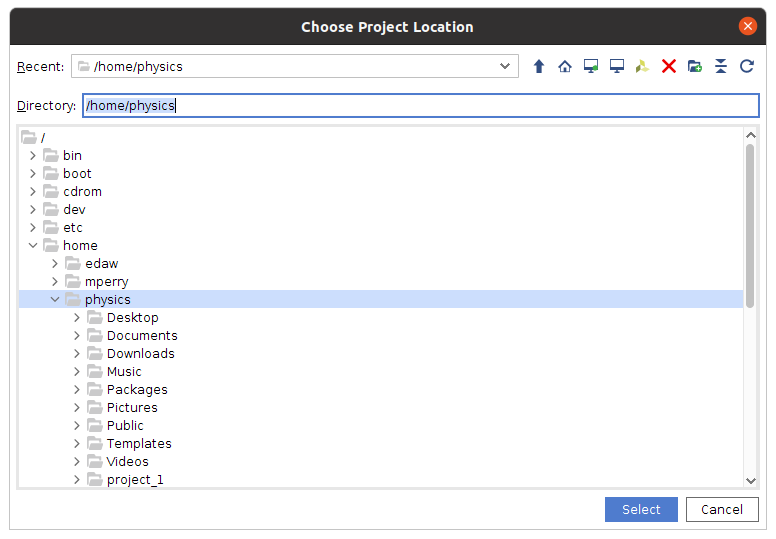
\includegraphics[width=0.5\textwidth]{figures/choose_project_location.png}
    \caption{Window to choose project location. The 'create folder' icon is the third from the right of the small icons in the top right hand corner of the window.}
    \label{fig:choose_project_location}
\end{figure}

The default location is your home directory. In this window, we can create a sub-directory of the currently selected directory (you'll see that physics, your home directory, is highlighted), by clicking the third icon from the right in the row of small icons in the top right hand corner of this window. Type \texttt{vivado\_projects} in this window and you will see a new folder with this name appears and becomes highlighted. Click Select. This returns you to the 'New Project' window, and you will see that the project location is now \path{/home/physics/vivado_projects}. Because you have the box checked that says `Create project sub-directory', Vivado will create a further sub-directory called \texttt{check\_leds\_and\_switches} within the Vivado projects directory. By using a new directory for every Vivado project we create, we can keep ourselves organised as we do more work. You are now done picking a project name and directory, so you can click the blue Next button ato the bottom, or use the shortcut alt-n. As an aside, in Vivado and many other software packages having graphical-user-interfaces (GUIs) every button that has a label with the first capital letter underlined has a keyboard shortcut of alt-(that key). No need to use shift because alt-n is the same as alt-N by convention. 

On the second page displaying in this window you keep the default which is 'RTL Project'.

On the third page you are asked to add sources. The sources are VHDL source files, and we are going to build ours from scratch, so you don't need to add any at this stage. So, Next (or alt-n) again. 

This brings you to the fourth page, where you are asked to add constraints. A constraint is a file that we will discuss further. It's basic functionality is to associate pins on the FPGA chip with ports, which are wires into and out of the circuit you are going to define in your VHDL code. We will always start with a standard constraint file that is supplied by Digilent, the makers of the BASYS3 board that we have lent you. You will find this file in your home directory, and it is called \texttt{Basys-3-Master.xdc}. You can add this constraint file now, or later on once the project is open. Let's add it now. Click on the '+' icon close to the top left of the window you are in, and select `Add Files...'. This will bring up a browser window, which is shown in Figure \ref{fig:add_constraint_file}.

\begin{figure}[htbp]
    \centering
    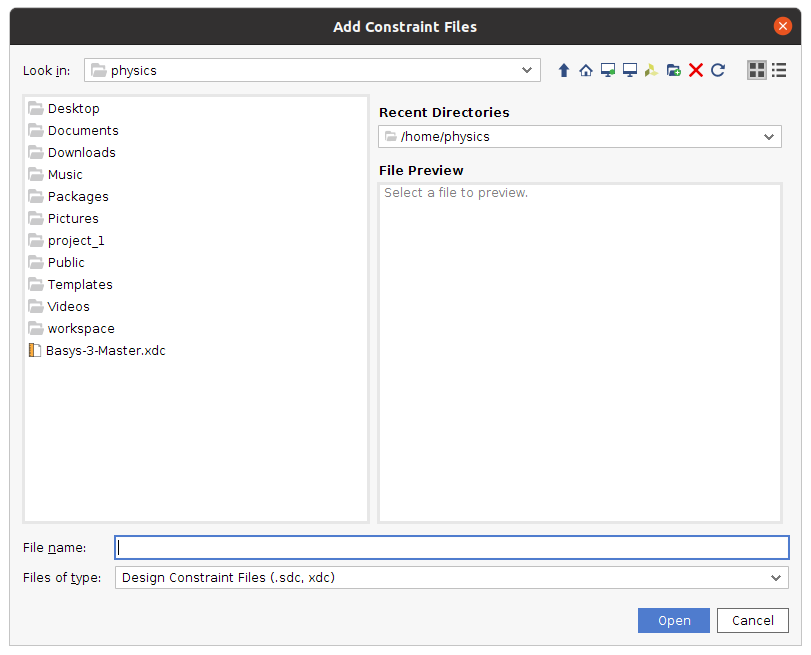
\includegraphics[width=0.5\textwidth]{figures/add_constraint_file.png}
    \caption{The browser window for selecting a constraint file.}
    \label{fig:add_constraint_file}
\end{figure}

The browser starts in your home directory by default, which is the location of the constraint file. Click on it, and the contents at the head of the file should appear in the `File Preview' pane to the right, and the file name should also appear in the box second from bottom of the window. Click OK, or just hit the Return key, and this should close the browser window. Finally, be sure to check the box in the bottom left hand corner that says `Copy constraints files into project'. This causes Vivado to duplicate the constraints file into a subdirectory of your project folder, so that you can re-use the generic one in your home directory for future projects. You don't have any more constraint files to add, so hit Next (or alt-n).

The next part of project specification is to select the Default Part, or sometimes you will instead want to select the Default Board. For today, we're just going to select the part. You'll see a long list of parts appear in a table in the lower part of this window. The list is so long that scrolling up and down it is a chore. The parts on this list are FPGA devices that is supported under your Vivado software license. One of these devices is the FPGA on the BASYS3 board, and as already mentioned the part number is \texttt{\bf xc7a35tcpg236-1}. Click in the Search window, (or alt-S) and type in the part number, and the list of parts in the table will narrow to just 1. Then, click on the one remaining row, and this part should be highlighted in blue. Note that in this table various statistics about the chip are given. It has 236 pins for input/output, 106 IOBs (input output buffers), 20800 LUT (look-up table) elements, 41600 FlipFlops, 50 block RAMs, 90 DSPs (digital signal processors), and you can use the horizontal scroll bar at the bottom to move across the table to see that it has 2 Gigabit transceivers and 2 GTPE2 transceivers, one PCIe (pci express module), 5 MMCM (multi-mode clock module), a minimum operating voltage of 0.95V, and a maximum operating voltage of 1.05V. Click next (or alt-n). This completes the specification of the project. Check that a new RTL project with the correct name of \path{check_leds_and_switches} will be created. Check that the default part is the one in bold above, of the Artix-7 family, package cpg236, and speed grade -1. Then, alt-f or click Finish. A small window indicating that some work is being done will appear and after that the Vivado window will change to the top window of the project. It might be best to use the 'square' icon in the top right of the window to maximise it to full screen. The window should appear as shown in Figure \ref{fig:vivado_project}.

\begin{figure}
    \centering
    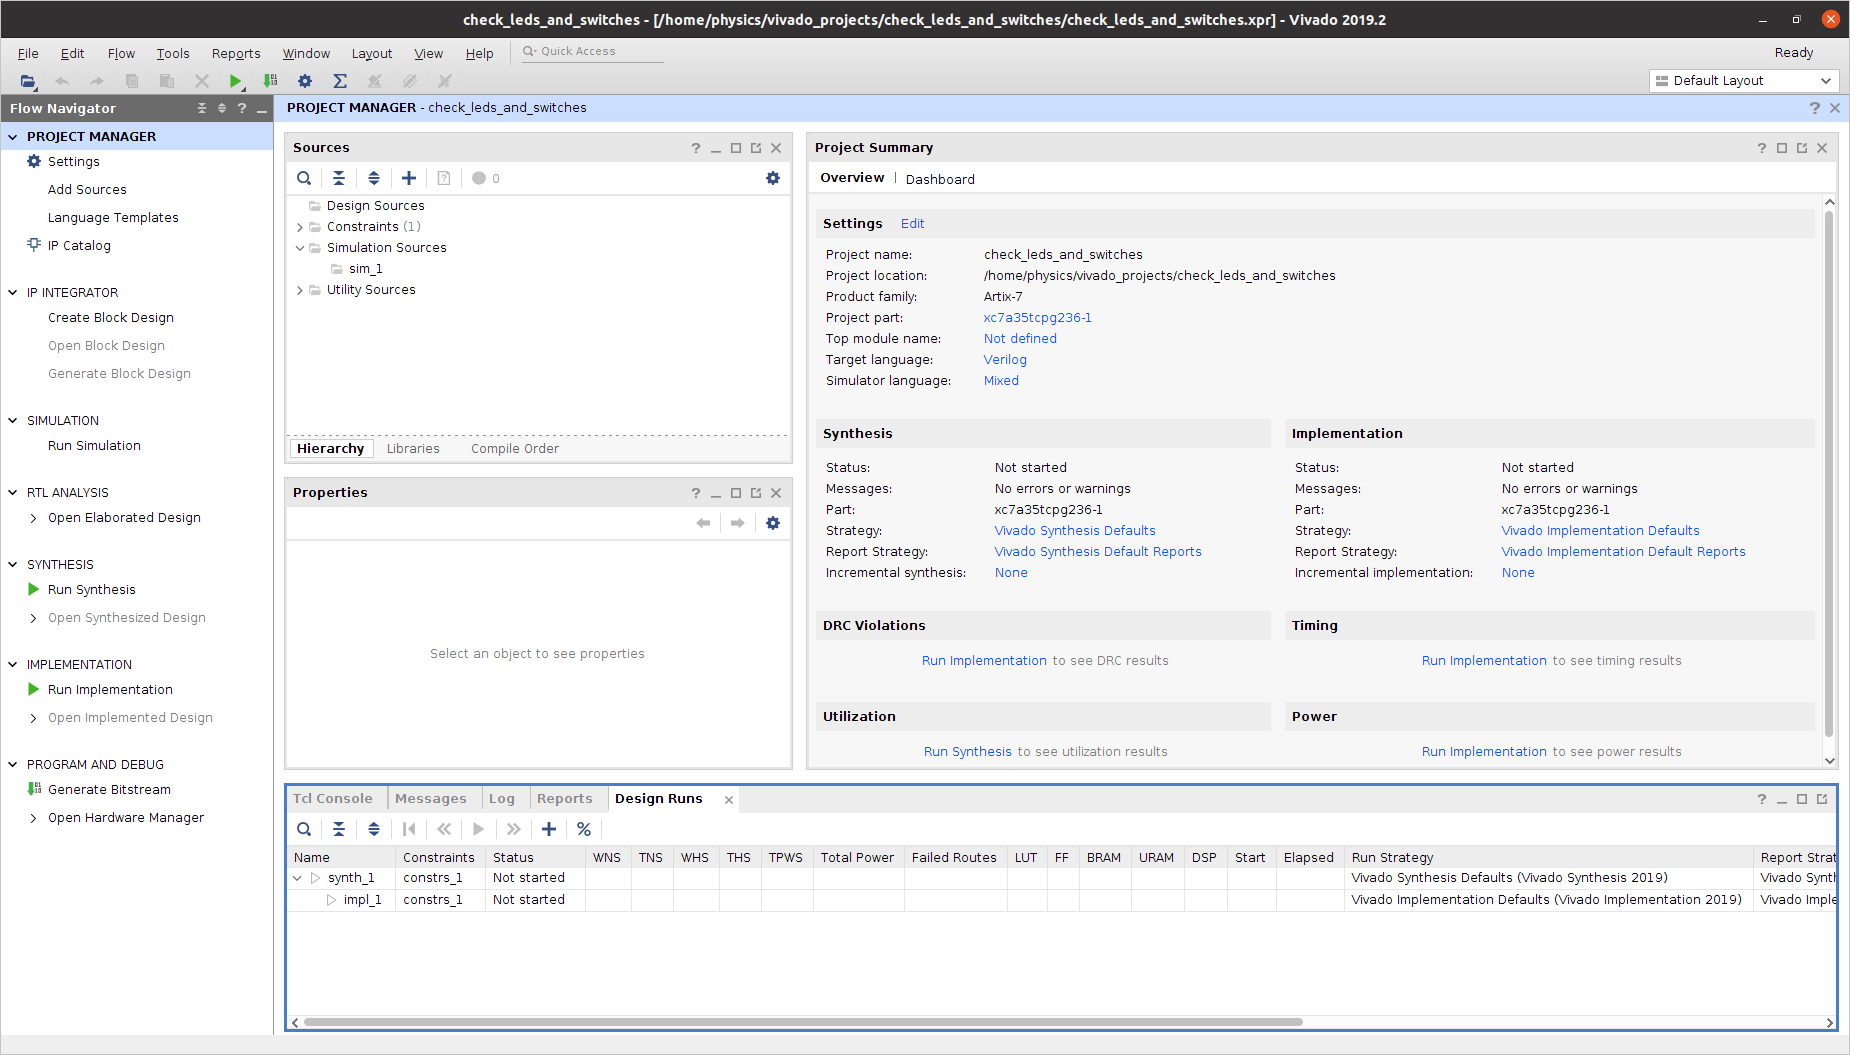
\includegraphics[width=\textwidth]{figures/create_new_vivado_project.png}
    \caption{A new Vivado project window on start-up.}
    \label{fig:vivado_project}
\end{figure}

\subsection{Organisation of the Vivado project window}
\label{sec:vivado_project_window}

The general layout is that there is a left hand `Flow Navigator' toolbar. This bar contains commmands, or directories (with a `$>$' on the left) containing more commands. At the top of this `Flow Navigator` on the right there is an underscore, which when you click on it causes the flow navigator to disappear. If this happens, you can make it reappear by clicking on the tall slim rectangle all the way on the left with `FLOW NAVIGATOR' written in it sideways. This should bring it back. The other three icons expand and collapse the contents of the `Flow Navigator', and give you some text help on what this navigator is for. 

The rest of the window consists of a set of panes, each of which have tabs in them. The biggest pane currently just has a `Project Summary' in it, which we will come to in a minute. To its left there are two smaller panes stacked vertically on top of each other. The top one says `Sources' and the bottom one says `Properties'. Each of these three panes has a cross in the top right hand corner. If you click on this, the pane disappears. If this happens, you can make it reappear by clicking on 'Window' in the top left of the Vivado project window and selecting the name of the pane. Try it with one of them.

At the bottom of the window is a long but squat pane with five tabs in it labelled 'Tcl Console', 'Messages', 'Log', 'Reports' and 'Design Runs'. Explore by clicking on them one-by-one. 

`Tcl Console' contains an enticing window with the words `Type a Tcl command here'. This is what is visible of the command line program underlying the graphical user interface (GUI). If you were an expert, you could run the entire SDK without ever using a mouse from this window. Indeed, many professional engineers probably do exactly that. As a point of interest, Tcl was a scripting language that was very popular in the 1990s and early 2000s, then fell out of favour, but not before the entire engineering community had bought heavily into it, rather in the same way that astronomers have gone a bundle for PYTHON. The Tcl language came with some rather nice GUI widgets so the package was called Tkl/Tk, and many GUIs, including earlier versions of Vivado, were built out of Tk widgets. So, that's why it's called a Tcl command. You'll never need it but it is nice to understand why things are the way they are. If you are curious, when we get to actually running commands, you can open up this Tcl Console window and view the actual command line tools that you have invoked by clicking on the symbols. This is why I know that you could run the whole program from the command line - all the GUI does is generate Tcl commands corresponding to the mouse clicks it detects, and then displays the results in a graphical format. It is literally a graphical interface to a command line, or shell, based tool.

The `Messages' tab is where you go to look for errors, warnings and information that are fed back to you after you run a command. You'll see that there are currently three messages of class info - if you uncheck the box they disappear, and if you recheck the box they come back. This is useful because if you run something and it goes wrong there may be 107 warnings of no interest and a single error that needs rectifying. By unchecking the `warnings' and `info' boxes you can view the error and do something about it.

`Log' shows all the text returned by all the commands you run in a single window. It is probably not a very efficient way of getting this information - you are better off with the `Messages' tab.

`Reports' is where you can view technical data about the products resulting from your design. Things like what fraction of the hardware resources on the chip are being used appear here.

`Design Runs' is where you can view progress when you launch a command that takes a few minutes to complete. One of the reasons that I lend out these laptops rather than having students install the software on their own machines is that Vivado and its underlying tools are actually very compute-intensive. These laptops were the best hard disk / processor / core combination I could find for the money. They are quite fast machines, but you'll still find yourself waiting for things, especially when the projects get more elaborate later in the course. You're probably best off leaving the 'Design Runs' tab open for now.

Each of the panes has a small icon in the top right hand corner to the left of the cross icon that hides the pane, which looks like a rectangle with an arrow in it. If you click this, it pulls the pane out into a separate window that you can make very large. Try this with one of them. If you want this window to go back into the Vivado project window, then next to the `X', the icon in this window now looks like a right angle with an arrow pointing southwest away from it. Click this and the window turns back into a pane. The next icon along in each pane is an empty rectangle. If you click this, that pane expands to fill a much bigger space, obscuring the other panes, but not the Flow Navigator. This is another way to concentrate on what is in one of the panes at the expense of the others. To reverse this action, click on the 'double square' icon that appears in the same place as the single square when you maximise the pane in this way. This will restore the pane you maximised to its previous size. There is also an `\_` icon which turns any pane into a tall thin rectangle at the edge, which you can retrieve by clicking on that rectangle. Try that too. Finally, each pane contains a '?' icon, which expands to some help on what that pane is for. In previous versions of the software this wasn't actually any use at all. However, it has improved, so do have a read of some of this help text.

All in all, I recommend that you spend some time exploring this SDK and how it is organised. Because you are all working remotely, if something wierd happens in the GUI, it will be far, far easier if you can make things right for yourself and not have to ask us to do it for you.

\subsection{Which hardware description language ?}
\label{sec:which_hdl}

There are two hardware description languages supported in Vivado - VHDL and Verilog. Verilog is probably used more extensively in professional engineering, but I think VHDL is a better language for first time hardware developers, because it makes very explicit certain concepts that are fundamental to the architecture of computers, particularly registers, which we will discuss next week. \texttt{Verilog} tries to look more like an ordinary high-level programming language like C, but I think that for a student this is actually counter-productive. So, we will use VHDL. If you look in your Project Summary window, however, you'll see that it says, on the left, amongst many other things, that the `Target language' is Verilog. This strange choice of words means - `I am expecting you to code in Verilog here'. We need to fix this or there's going to be trouble. So, click on the blue 'Edit' in this pane, click on the arrow next to Verilog in the window that appears, and select VHDL instead, followed by OK. Now you are set up to compile VHDL code in Vivado.

As an aside, after I started learning about VHDL for myself about a decade ago, I realised that it reminded me of a work experience placement I had when I was at school, at a company called Lucas Aerospace. The engineers there sent me off to write code for a PAL, which stands for programmable array of logic, in a language called ABEL. I ended up concluding that the PAL the engineer had selected didn't have enough gates on it to implement the functionality that the engineer wanted, so it wasn't a roaring success. Well, it turns out that a few years later Xilinx bought ABEL, and used it as the precursor to developing VHDL. So, without realising it, I have been programming in hardware description languages since I was fifteen! And, it turns out that ABEL is still in use, in some quarters, 35 years later. All that happened is the devices got bigger - PALS became CPLDs (complex programmable logic devices) which then got even larger and became FPGAs, and now we have SoCs, which are systems-on-a-chip. What's next? Maybe UoS, which instead of University of Sheffield could be Universe-on-Silicon ?

\subsection{A first look at the constraint file}
\label{sec:constraint_file}

In the `Sources' pane, there is a folder icon with Constraints (1) written next to it. Click on the `$>$' next to that folder. The folder hierachy should expand and the file Basys-3-Master.xdc that you incorporated as a constraint file should appear. Double click on this file. It opens in the largest pane (which I'll just call the main pane from now on) as a new tab. There should now be two tabs in the main Pane, the constraint file and the `Project Summary' tab that was there before. Use the mouse to toggle between views of the two tabs. Go back to the constraints tab. Scroll up and down inside the file and take a look at its contents.

First, note that every single entry in this file, with the exception of a couple at the end, starts with the `\#' character. This is the comment character in constraint files, so before we start doing things every line in this file is commented out. However, if you look down this file whilst also looking at the board you'll begin to notice a correspondence between the constraint file entries and the hardware. Here are some observations I would make.

\begin{itemize}
    \item The file entries are divided into blocks with space lines between the blocks.
    \item The first block below the four comment lines at the top is to do with a Clock signal. We won't worry about clocks this lab.
    \item After this there is a block entitled Switches. The lines in this block are in pairs. The first line of each pair contains a letter-number combination. In the first pair it is V17, in the second it is V16, etc.
    \item There are 16 of these pairs in the switches block.
    \item There are 16 switches on the board. If you look at the board, can you find the letters V17, V16, and the other similar pairs printed on the board in the vicinity of the switches?
    \item Moving past the switches block, the next block says LEDs. This block too has pairs of lines, and there are 16 pairs in all.
    \item Like the switches, the LED lines are associated with alphanumeric codes, like U16 and E19. Look at the board and locate the LEDs, close to the switches, that have these alphanumeric codes next to them.
\end{itemize}

We're actually only going to use the LEDs and switches today, so you don't need to worry about the remainder of the constraint file. However, if you want to take a quick look, the remaining blocks also correspond to physical devices connected to the FPGA. For example, the 3 blocks below the title 7 segment display, with 7 pairs of lines then a space then a pair of lines on its own, then four more pairs of lines, are all related to the four digit alphanumeric LED display on the board. The five pairs labelled Buttons correspond to the cluster of five pushbuttons - notice the names of the ports are btnC (central), btnU (up), btnL (left) ...etc, corresponding to the physical arrangement of the buttons on the board. The four groups labelled Pmod Header JA, JB, JC, and JXADC have to do with the four 12-pin expansion connectors, or PMOD connectors, on the two short sides of the board. The section labelled VGA Connector corresponds to the pins of the micro-D connector on the back side, which is designed to control an analog RGB monitor. The remaining blocks are associated with an RS232 serial interface that can be connected to the micro-USB connector next to the on switch, the full sized USB port in the top right corner, and some SPI flash memory connected to the FPGA.

\subsection{Modifying the constraint file}
\label{sec:constraints}

Remember from the first lecture (see Chapter \ref{sec:chapter1_logic_integers}) when I discussed buses? In this constraint file, the LEDs and switches are each configured as 16 bit wide buses. You have a bank of 16 switches and a bank of 16 LEDs. Each LED and each switch is wired to a different physical pin on the FPGA hardware. The FPGAs have a grid of pins that cover the whole back side of the chip, except for a square in the centre that for this chip has no pins. The pins are arranged in a square grid. These alphanumeric codes are literally the grid references of the pins that are connected to the devices in question. After these alphanumeric codes are square brackets containing syntax like `get ports \{sw[0]\}'. A port is VHDL syntax for the name of an input and output in the hardware description language. Where an input or an output is part of a bus, the square brackets specify which bit this port is. So, in the case of this port, it's the least significant bit, bit 0, of the 16 bit bus connected to the switches. Looking down the rest of the switches, you can see that each pair of lines refers to a different bit in the bus, from the LSB at the top to the MSB at the bottom. The second line in each pair specifies what type of voltage standard the hardware is - in this case LVCMOS33 means low voltage CMOS 3.3V. These lines are used when Vivado is doing timing simulations on the signals propagating across the FPGA. 

You are going to need to uncomment all the lines in the switch and LED blocks. To do this, use the left mouse button to highlight the entire block, or as much of it as you can at once. The lines you highlight will turn blue. At the top of the Basys-3-Master.xdc tab, there are 11 small icons. The third from the right is `//'. If you click on this it will uncomment the highlighted lines. They should change from grey to black and blue, and the comment characters at the beginning of the lines should disappear. Carry on with this until you have uncommented all the lines in the switch and LED blocks, except the first line in each block, where the double comment character is a way of telling you that this is just a title.

After uncommenting all the switch and LED blocks, you'll need to save changes. Notice that after you started altering the constraint file, an asterisk (star) appeared next to the file name at the top of the tab. This means the file has unsaved changes. To save these changes, hold down the Ctrl key and press s (ctrl-s). The asterisk should disappear when your changes are saved. Your constraint file is now ready to use.

\subsection{Creating a source file}
\label{sec:sourcefile}

Our next job is to create our VHDL source file. To do this look in the `Flow Navigator' sidebar and click `Add Sources'. A window appears, with three options, the middle of which is 'Add or create design sources'. Click the button next to this option to select and then click Next. The ensuing window looks a lot like the one where you added the constraint file earlier. In fact, it's the same window, only this time, we don't want to add an existing file, we want to create one from scratch. To do this, click the plus sign towards the top left corner and select `Create File'. A sub-window appears. The file type should be VHDL, but you need to give the file a name. Click in the box next to File name. It can be anything you want as long as it ends in .vhd, only don't include any spaces in the name. How about `switch\_to\_led.vhd'. That is what I called mine, anyway. Hit OK. This should return you to the `Add Sources' window, and your file should be visible as shown in Figure \ref{fig:add_sources}

\begin{figure}[htbp]
    \centering
    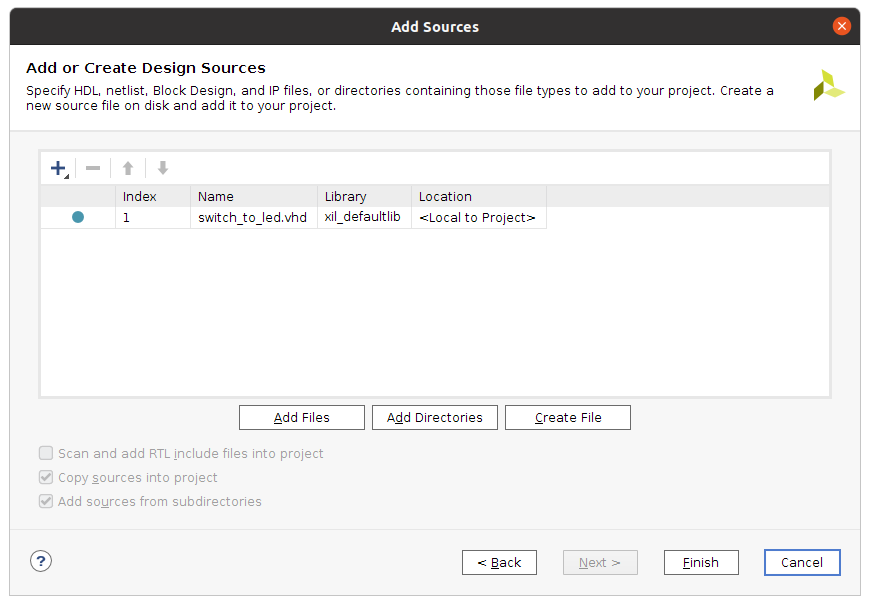
\includegraphics[width=0.5\textwidth]{figures/add_sources.png}
    \caption{The `Add Sources' window after you have named your source file.}
    \label{fig:add_sources}
\end{figure}

You can now click Finish, only it's not over yet. A new window appears called 'Define Module'. You don't actually have to use this, but it is quite useful to do so as it gets your source code off to a good start. In this window there is a table called I/O Port definitions. In our module, there will be an input port bus for the signals from the 16 switches and an output port bus for the signals going to the 16 LEDs. So, in the top left cell just under port name, click in the box and write sw, which if you recall was the name of the 16 ports for the switches in the constraint file. Check the box to confirm that this input is a Bus. Next click on the zero in the MSB column. The zero is now blue and you can just enter 15, or click the up arrow until the zero increments to 15. As long as it ends up as 15, that's OK. 

Next click in the next row down directly below where you wrote sw. The row fills with entries. Click again and then you can enter led as the port name. Change the `in' to `out' on this row as the switches are outputs, check the Bus box again, and change the MSB to 15. Click OK to finish. In the Sources pane, you should now be able to see your file under `Design Sources' with whatever filename you gave it. Double click on the file name and your file will open up in the main pane. Now you have three tabs in the main pane - Project Summary, Basys-3-Master.xdc, and your VHDL source file.

\subsection{Modifying the source file}
\label{sec:source_file_mods}

The first thing you'll notice about the source file when you open it is that most of the lines begin with two dashes in a row. This is the comment character in VHDL. It is a bit annoying that the VHDL comment character is different from that in the constraint file. It's because the constraint file syntax is actually Tcl syntax, and I believe the double dash comment character originates in the ABEL language I used when I was 15! The file lines are numbered, and everything up to and including line 21 is basically superfluous. I suggest that you delete these lines. Line 22 is the first important one, where it says `library IEEE;'. You can also remove the remaining comments after `use IEEE.STD\_STD\_LOGIC\_1164.ALL' and 'entity switch\_to\_led is'. The code should now look like this.

\newpage

\begin{minted}{vhdl}
----------------------------------------------------
--- WARNING - THIS CODE WILL NOT BUILD UNTIL -------
--- YOU MAKE THE ADDITION GIVEN ON THE NEXT PAGE ---
----------------------------------------------------
library IEEE;
use IEEE.STD_LOGIC_1164.ALL;

entity switch_to_led is
    Port ( sw : in STD_LOGIC_VECTOR (15 downto 0);
           led : out STD_LOGIC_VECTOR (15 downto 0));
end switch_to_led;

architecture Behavioral of switch_to_led is

begin


end Behavioral;
\end{minted}

Here is an explanation of the code. The first couple of lines declare that you will be using logical data types. The four lines starting with entity switch\_to\_led is and ending with end switch\_to\_led describe the input and output ports to your logic circuit. In this case, we have a 16 element input bus whose port name is sw, and a 16 element output bus whose port name is led. Notice that sw and led match the port names in the constraint file. It is very important that this is so, otherwise the code will not compile correctly. Notice that the ports are defined between a pair of round brackets, and the two port declarations are separated by a semicolon. Notice also that the last port declaration has a semicolon OUTSIDE the round bracket that encloses the ports, but no semicolon inside this bracket. All this syntax is correct, and the ports are already correctly defined because we used the GUI window during the create source sequence to specify our ports ahead of time.

VHDL differs from python in that it does not use whitespace characters like spaces, tabs or newlines to convey information. A command is terminated by a semicolon. You can have as much whitespace as you like in a single statement, so long as use a semicolon to tell the compiler when that statement is finished. Personally I think this is profoundly sensible. But, it does mean you have to be careful to remember the semicolons.

What is still missing is what connects the input ports to the output ports. All we want to do to start with is connect each of the 16 switches to the corresponding LED. To do that we add one line as follows:

\newpage

\begin{minted}{vhdl}
library IEEE;
use IEEE.STD_LOGIC_1164.ALL;

entity switch_to_led is
    Port ( sw : in STD_LOGIC_VECTOR (15 downto 0);
           led : out STD_LOGIC_VECTOR (15 downto 0));
end switch_to_led;

architecture Behavioral of switch_to_led is

begin
    led <= sw;
end Behavioral;
\end{minted}

The architecture part of the code is where you define how your circuit is connected together between the ports. In this case, it is very simple. We just connect the 16 bit input bus from the switches to the 16 bit output bus going to the LEDs. The $<=$ operator is the 'assignment' operator that makes the connection. It is formed from a less than sign followed by an equals sign. Do not get confused and write just $=$ in this context. That means something else in VHDL. Think of $<=$ as wires connecting two objects. Use ctrl-s to save your file.

Vivado has an automatic syntax checker. If you have made the file correctly, the file name should remain in bold in the Design Sources window. If however you have made a syntax mistake, this will be indicated in your `Sources' pane as shown in Figure \ref{fig:syntaxerror}.

\begin{figure}[htbp]
    \centering
    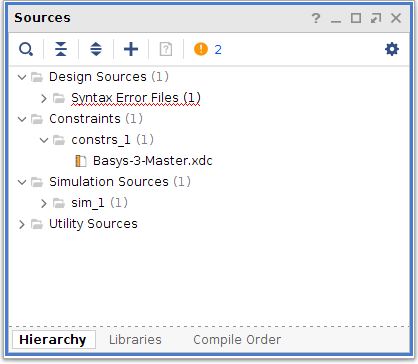
\includegraphics[width=0.5\textwidth]{figures/syntax_error.png}
    \caption{Appearance of the `Sources' pane when Vivado has found a syntax error in a VHDL source file.}
    \label{fig:syntaxerror}
\end{figure}

Even if you didn't make any errors, try inserting a rogue character in your VHDL file, then using ctrl-s to save, so that you trigger the error checker. If you click on the `$>$' next to Syntax Error Files, your file is there, and it is not highlighted. Now fix the error and ctrl-s again, and your file is restored to Design Sources and is listed in boldface. Vivado's editor also spots syntax errors in-line by underlining them in red. If you see this kind of red underlining in your file, it probably means you should look for a mistake.

\subsection{Synthesising your design}
\label{sec:synthesis}

You are now ready to run synthesis on your design. In this step, Vivado and its underlying compiler determine the optimal set of logical entities available on the chip to implement your circuit. Of course, this design will use very few resources, but it's our first one, so no surprises there. Click `Run Synthesis' in the `Flow Navigator' bar on the left. When you do this, a small 'Launch Runs' window appears. This is shown in Figure \ref{fig:launch_runs}. 

\begin{figure}[htbp]
    \centering
    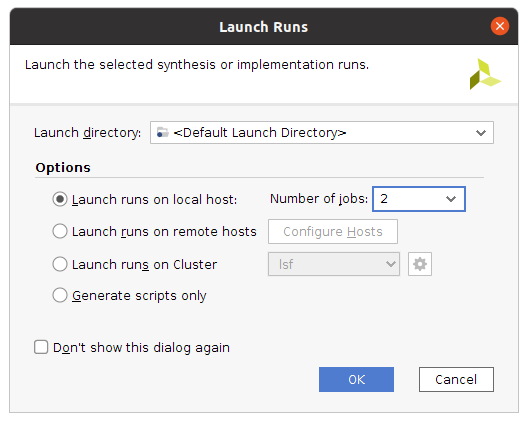
\includegraphics[width=0.4\textwidth]{figures/launch_runs.png}
    \caption{The `Launch Runs' window}
    \label{fig:launch_runs}
\end{figure}

This window isn't so important for this simple job, but for larger jobs you can save significant time here. Vivado is capable of operating multiple CPU cores at once. In this window you can select a number of jobs up to 4. This means that you can use up to the 4 cores that your laptops i7 pentium processor has. Where you are building multiple modules at once, this will literally divide your build time by four. So, it's well worth being aware of this functionality. In this case just hit OK.

If all goes well, you will see a small `Synthesis Completed' window like the one in Figure \ref{fig:synthesis_completed}. 

\begin{figure}[htbp]
    \centering
    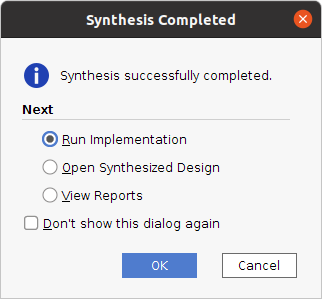
\includegraphics[width=0.4\textwidth]{figures/synthesis_completed.png}
    \caption{The `Synthesis Completed' window}
    \label{fig:synthesis_completed}
\end{figure}

You next want to launch the `Run Implementation' step. This step figures out how to route the wires between the input and output pins on the chip and the required logical elements. Just select OK to start this process. Again, the default of 2 parallel jobs is OK for this build. You'll have to wait a short while for this to complete. If everything goes well, you should see another similar window, 'Implementation Completed'. This time you want to skip opening the implemented design, so just select 'Generate Bitstream', and then click OK (or hit return). Once the bitstream has built, a 'Bitsream Generation Completed' window appears. In this window, you just hit cancel, because we need to get the board hooked up before we launch on the hardware.

\subsection{Launching on hardware}
\label{sec:launchingonhardware}

We are now ready to launch on the hardware. The first step is to connect the BASYS3 board to the computer. Before we do this, however, there are a few checks. On this board, in the top left and top right corners there are some blue 'jumpers' connected across pairs of pins. The jumper in the top left (with the switches at the bottom) should be connected between the middle of the three pins and the one towards the inside of the board, with the letters `USB' written on the board next to it. This jumper sets the board to be powered from your laptop through the USB cable. The other jumper position instead draws the board power from the two pins below the power switch labelled EXT and GND. The power switch itself should be in the `OFF' position, with the switch slid towards the inside of the board. 

The other jumper next to the big USB port should be set in the middle position it can occupy, connecting the middle two of the four pins. The board can be programmed in three ways, and the way we will be using today is to program the board directly from an external device by way of a so-called JTAG chain. A JTAG chain is a standard protocol for programming multiple chips through a serial interface. The other two programming methods are to program the board from an on-board flash memory chip (QSPI) and from a USB stick plugged in to the large USB port (USB). 

The computer connects to the board using the usb to microusb cable that I supplied you with. Ensure the board is not on a metallic surface that could short out the pins. Note that the micro USB plug connects to the BASYS3 with the flat and larger side of the D connector UPWARDS. Do not force it in because these connectors are not all that robust! It should go in quite easily. Connect the board up to any USB port on the laptop and turn it on at the switch. A red light in the top left hand corner of the board should light up, and an orange light next to the large USB port should come on for a second or so, and then go out.

Back in Vivado, at the very bottom of the `Flow Navigator', click on the arrow next to `Open Hardware Manager'. Click on `Open Target', and select `Open New Target...'. A window will appear called `Open New Hardware Target'. Click next. On the next screen, you want to accept the default that your target is connected to your local machine, so click next again. The window should now show your Digilent device as a hardware target. This is shown in Figure \ref{fig:hardware_target}. Click Next and then Finish.

\begin{figure}[htbp]
    \centering
    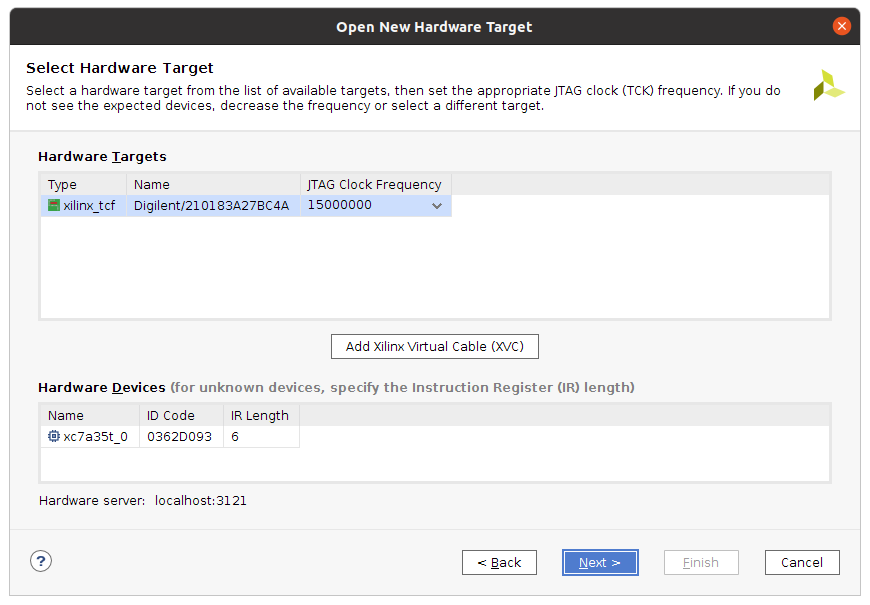
\includegraphics[width=0.7\textwidth]{figures/hardware_target.png}
    \caption{The hardware window with the digilent board and device visible.}
    \label{fig:hardware_target}
\end{figure}

\subsection{Programming the device}
\label{sec:programming}

You should now be able to program the board. At the bottom of the `Flow Navigator' sidebar, click on `Program Device' and select the xc7a35. In the window that appears, you can see the bitstream file, switch\_to\_led.bit, which is used to program the chip. Click program, and after a few moments, the green LED in the top right hand corner of the board indicates that programming is `done'. Operate all the switches and verify that the corresponding LED lights up when any switch is thrown. Make a note of any that do not work.

\subsection{The hardware manager}
\label{sec:hardware_manager}

Once you have the hardware device programmed, your Vivado window will have changed to a state where the `hardware manager' is running and visible. The appearance of the Vivado window in this state is shown in Figure \ref{fig:hardware_manager}. 

\begin{figure}[htbp]
    \centering
    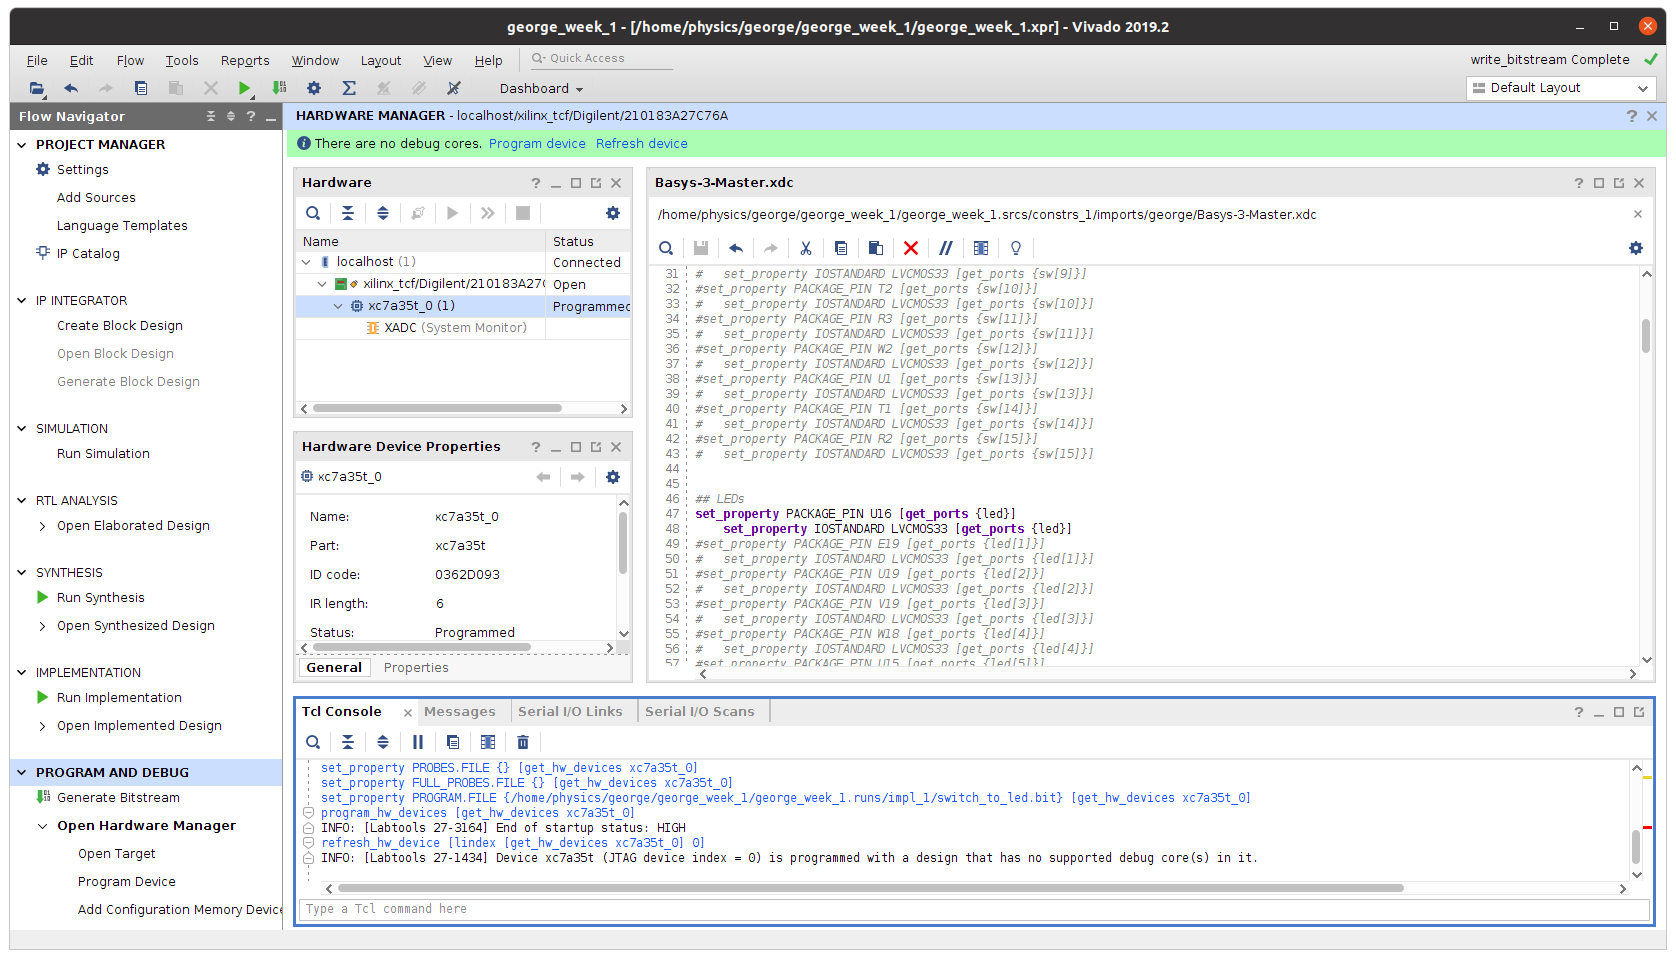
\includegraphics[width=\textwidth]{figures/hardware_manager.png}
    \caption{The Vivado window when the hardware manager is open}
    \label{fig:hardware_manager}
\end{figure}

In this state, the chip is being monitored in real time by Vivado. The Artix7 has an on board temperature sensor and analog-to-digital converter, so it can measure its own temperature. This is so that commercial applications can put in safeguards for overheating - which is why your mobile phone will probably switch itself off if you leave it on a sunny windowsill in the summer. If you double click on XADC in the Hardware pane, then click `OK' in the`New Dashboard' window that appears, this will bring up an updating strip chart of the measured temperature of the FPGA in centigrade. You can put your finger on the chip and after a while you will start to see it warm up. 

If you turn off or disconnect the board with the hardware manager on, a window will come up informing you that it has lost the connection to the device. This can also happen if your USB cable isn't very well connected at either end, or when you pick the board up with the cable hanging off the connector. It's fine just to click OK if this happens. If you wish to reconnect to the board, just turn it back on, plug the cable back in, or fix whatever the hardware issue was, then at the top of the hardware manager board you can click on `Open target', then select `Auto Connect'. It should re-connect to the board when you do this. You will then have to re-program the board using the instructions in Section \ref{sec:programming}. 

Once you are done with studying your hardware, you may want to start over with a new project, or make modifications to the one you have open. Before doing this, click the `X' in the hardware manager pane to close it, and then confirm that you want to close it with `OK'. This will take you back to the more regular appearance of the Vivado window so you can proceed with further modifications, or close the project and create a new one.

\subsection{Other project ideas}
\label{sec:other_ideas}

Here are some other projects you might try. Some of them are very modest modifications to the project already described. Others are more substantial new work. Remember that whenever you modify the constraints file or any of the VHDL code in your projects, you must use ctrl-s to save the changes to your files, at which point the asterisks next to their names should disappear, then redo the process of synthesis, implementation and bitstream generation. Note that you can take a short-cut by clicking on `Generate Bitstream', which will cause it to synthesise and implement as well, after it prompts you to confirm that it's okay for that to happen. This saves you effort, but it also means that if something goes wrong it may be less obvious to you at which stage it failed.

One additional piece of advice. In my experience more than half of student mistakes have to do with syntax errors in the constraint file, usually with the various square brackets and curly braces. Double-check that you haven't left any stray braces lying around as they are hard to spot in the generally cluttered syntax of these files. If your constraint file is faulty, this may cause the build to fail at the last stage when Vivado is generating the bitstream. This is a clue that can help you go back and give the constraint file extra scrutiny.

For the projects that require quite major changes to the VHDL code and constraints, you might be better off starting again with a new project. To do this you can either close the project you are currently working on using \texttt{File->Close project} from the file menu, or much as you can do in WORD or EXCEL, you can instead use \texttt{File->Project->Save As...}. The latter will create a copy of your current project, allowing you to select the project location, which should certainly be \texttt{/home/physics/vivado\_projects}, and a new project name, which should suit whatever the modified project is going to do. This way your current functioning project remains intact, but you avoid having to set up a new project from scratch, since you can now go on to modify the copy without losing the original.

After all that, here are some ideas for other projects you could usefully work on.

\begin{enumerate}
    \item Change to 
\begin{minted}{vhdl}
    led <= not(sw);
\end{minted}
    so that the LEDs are off when the switches are on.
    \item Make the bottom 8 switches control the top 8 LEDs and vice versa. To do this, use the downto mechanism to refer to a subset of the lines of a bus, so
\begin{minted}{vhdl}
    led(7 downto 0) <= sw(15 downto 8);
    led(15 downto 8) <= sw(7 downto 0);
\end{minted}
    \item Change the constraint file so that only two of the switches and one LED are enabled. Do this by commenting out all the others. But, also, name the switches and the LED as separate discrete ports instead of elements of a bus. So, for example, where the constraint file currently says
\begin{minted}{tcl}
set_property PACKAGE_PIN W16 [get_ports {sw[2]}]
	set_property IOSTANDARD LVCMOS33 [get_ports {sw[2]}]
\end{minted}
    you should modify each of the two switches left so it is a discrete one-element bit rather than a bus element, as follows
\begin{minted}{tcl}
set_property PACKAGE_PIN W16 [get_ports {swone}]
	set_property IOSTANDARD LVCMOS33 [get_ports {swone}]
\end{minted}
and similarly for the two lines corresponding to the other switch. In your VHDL code, you need to declare the switch as a separate port, so if the new names of your two switches are swone and swtwo and your single LED is just named led, then your VHDL code port section becomes
\begin{minted}{vhdl}
entity switch_to_led is
    Port ( swone : in STD_LOGIC;
           swtwo : in STD_LOGIC;
           led : out STD_LOGIC);
end switch_to_led;
\end{minted}
Notice that once the inputs and outputs are no longer buses but single bits, the data type changes from STD\_LOGIC\_VECTOR to STD\_LOGIC. Now that you have simpler discrete inputs and outputs, try the logic gates, so that in the architecture portion of your code you could write
\begin{minted}{vhdl}
architecture Behavioral of switch_to_led is
begin
    led <= swone xor swtwo;
end Behavioral;
\end{minted}
Check that the logic gates have the correct behaviour.
\item 
Work out a simple set of logic gates that implement a one bit adder with carry. The functionality should be, when both the inputs are zero, the output is zero and the carry is zero. When one of the inputs is one and the other is zero, the output is one but the carry is zero. When both the inputs are one, the output is zero and the carry is one. Both the output and the carry are displayed on LEDs. Design your logic to implement this simple adder, and build and test your design on your board.
\item 
Implement a one bit adder, but this time it needs to have three inputs, one for each of the two inputs to the one bit adder you already designed, and a third input to accept any bits carried over from another column. You'll need to figure out a truth table for the two outputs, the out for this bit and the carry out for the next one, from the three inputs, then enable three switches and two leds to test whether your logic implements the truth table, reprogram the board and test your hardware.
\end{enumerate}

\end{document}